% !TeX program = xelatex
% !TeX root = main.tex
% Báo cáo Bài tập lớn ShopFlash, môn Hệ quản trị Cơ sở dữ liệu (HK261, lớp L01).
% Dựa trên hcmut-report-template (MIT, (c) 2026 Thuan Nguyen Minh, xem TEMPLATE_LICENSE),
% chuyển sang XeLaTeX để ghép được nội dung có ký tự Unicode và code có chú thích tiếng Việt.
% Cách biên dịch và quy ước file cho từng người: report/AGENTS.md.
\documentclass[12pt, a4paper, oneside]{article}

% ---------- Thông tin trang bìa: sửa ở đây ----------
\newcommand{\khoa}{KHOA ..........}
\newcommand{\monhoc}{HỆ QUẢN TRỊ CƠ SỞ DỮ LIỆU}
\newcommand{\detai}{..........}
\newcommand{\lop}{L01}
\newcommand{\nhom}{..}
\newcommand{\hocky}{Học kỳ ..........}
\newcommand{\giangvien}{..........}
\newcommand{\noivathoigian}{Thành phố Hồ Chí Minh, tháng .. năm ....}

% ---------- Font và tiếng Việt (XeLaTeX) ----------
\usepackage{fontspec}
\IfFontExistsTF{Times New Roman}{\setmainfont{Times New Roman}}{\setmainfont{TeX Gyre Termes}}
\IfFontExistsTF{Consolas}{\setmonofont{Consolas}[Scale=0.9]}{%
  \IfFontExistsTF{Latin Modern Mono}{\setmonofont{Latin Modern Mono}}{%
    % File names also work when a container user's fontconfig cache is missing.
    \setmonofont{texgyrecursor-regular.otf}[
      BoldFont=texgyrecursor-bold.otf,ItalicFont=texgyrecursor-italic.otf,
      BoldItalicFont=texgyrecursor-bolditalic.otf,Scale=0.9]}}
\usepackage{scrextend}
\changefontsizes{13pt}
% Không ngắt từ: mẫu ngắt từ tiếng Anh cắt sai âm tiết tiếng Việt.
\hyphenpenalty=10000
\exhyphenpenalty=10000
\emergencystretch=3em

% ---------- Trang, đoạn ----------
\usepackage[left=40mm, right=25mm, top=40mm, bottom=25mm]{geometry}
\usepackage{setspace}
\usepackage{indentfirst}
\setlength{\parindent}{1.25cm}

% ---------- Gói dùng chung. Phần nội dung của từng người không tự \usepackage ----------
\usepackage{amsmath,amssymb}
\usepackage{enumitem}
\usepackage{graphicx}
\usepackage{multirow}
\usepackage{array}
\usepackage{tabularx}
% Cột chữ căn trái cho bảng: L (co giãn như X), P{độ rộng}. Không ngắt từ nên cột hẹp căn đều sẽ giãn chữ.
\newcolumntype{L}{>{\raggedright\arraybackslash}X}
\newcolumntype{P}[1]{>{\raggedright\arraybackslash}p{#1}}
\usepackage{booktabs}
\usepackage{float}
\usepackage{caption}
\usepackage{subcaption}
\usepackage{xcolor}
\usepackage{tikz}
\usetikzlibrary{shapes.geometric, arrows.meta, positioning, calc}
\usepackage{pgfplots}
\pgfplotsset{compat=1.18}
\usepackage{listings}
\usepackage{fvextra}
\fvset{breaklines=true}
\usepackage{pdfpages}
\usepackage{fancyhdr}
\usepackage{titlesec}
\usepackage[backend=biber, style=ieee]{biblatex}
\usepackage{xurl}
\usepackage{hyperref}

% ---------- Tài liệu tham khảo: file chung và file của từng chủ đề (nếu có) ----------
\addbibresource{references.bib}
\newcommand{\nguonchude}[1]{\IfFileExists{#1/#1.bib}{\addbibresource{#1/#1.bib}}{}}
\nguonchude{storage}
\nguonchude{indexing}
\nguonchude{query}
\nguonchude{transaction}
\nguonchude{concurrency}
\nguonchude{backup-recovery}

% ---------- Ảnh: tên file phải khác nhau giữa các chủ đề (bắt đầu bằng số mục, ví dụ 3.5-01-...) ----------
\graphicspath{{figures/}{storage/images/}{indexing/images/}{query/images/}{transaction/images/}{concurrency/images/}{backup-recovery/images/}}

% ---------- Tiêu đề mục ----------
\setcounter{secnumdepth}{3}
\setcounter{tocdepth}{2}
% Tiêu đề mục in hoa, cỡ 14, canh giữa (lệnh cuối của tham số cuối nhận nội dung tiêu đề).
\titleformat{\section}[block]
  {\centering\normalfont\fontsize{14pt}{16.8pt}\selectfont\bfseries}
  {\thesection}{0.5em}{\MakeUppercase}
\titleformat{\subsection}[hang]{\normalfont\normalsize\bfseries}{\thesubsection}{0.5em}{}
\titleformat{\subsubsection}[hang]{\normalfont\normalsize\bfseries\itshape}{\thesubsubsection}{0.5em}{}
\renewcommand\thesection{\arabic{section}.}
\renewcommand\thesubsection{\arabic{section}.\arabic{subsection}}

% ---------- Chú thích hình, bảng, code; tên gọi tiếng Việt ----------
\captionsetup[table]{position=top, labelfont=bf, textfont=it, font=small, skip=5pt}
\captionsetup[figure]{position=bottom, labelfont=bf, textfont=it, font=small, skip=5pt}
\captionsetup[lstlisting]{labelfont=bf, textfont=it, font=small}
\renewcommand{\figurename}{Hình}
\renewcommand{\tablename}{Bảng}
\renewcommand{\lstlistingname}{Mã}
\renewcommand{\contentsname}{\centering MỤC LỤC}
\renewcommand{\listfigurename}{\centering DANH SÁCH HÌNH}
\renewcommand{\listtablename}{\centering DANH SÁCH BẢNG}

\hypersetup{
  colorlinks=true, linkcolor=black, citecolor=black, urlcolor=blue!50!black,
  pdftitle={Báo cáo Bài tập lớn \monhoc},
  pdfauthor={Nhóm \nhom, lớp \lop},
}

\pagestyle{fancy}
\fancyhf{}
\renewcommand{\headrulewidth}{0pt}
\fancyfoot[C]{\thepage}
\setlength{\headheight}{15pt}

% Kiểu chèn code dùng chung, được \input trong main.tex.
% Dùng: \begin{lstlisting}[language=OracleSQL, caption={...}, label={lst:cc-...}] ... \end{lstlisting}
% Ngôn ngữ có sẵn: OracleSQL, Redis, Lua, Java, Python, bash. Đoạn chỉ là văn bản thì dùng Verbatim (fvextra).
\definecolor{codebg}{RGB}{248,248,248}
\definecolor{codecomment}{RGB}{0,120,0}
\definecolor{codekeyword}{RGB}{0,0,170}
\definecolor{codestring}{RGB}{163,21,21}
\definecolor{codenumber}{RGB}{128,128,128}

\lstdefinestyle{shopflash}{
  basicstyle=\ttfamily\small,
  backgroundcolor=\color{codebg},
  commentstyle=\itshape\color{codecomment},
  keywordstyle=\bfseries\color{codekeyword},
  stringstyle=\color{codestring},
  numbers=left, numberstyle=\tiny\color{codenumber}, numbersep=6pt,
  frame=single, rulecolor=\color{black!25},
  breaklines=true, columns=fullflexible, keepspaces=true,
  showstringspaces=false, upquote=true, tabsize=2,
  captionpos=t, aboveskip=6pt, belowskip=6pt
}
\lstset{style=shopflash}

% SQL của Oracle: thêm các từ khóa SQL chuẩn của listings chưa có.
\lstdefinelanguage{OracleSQL}[]{SQL}{
  sensitive=false,
  morekeywords={MERGE,USING,MATCHED,NOWAIT,SKIP,LOCKED,WAIT,SERIALIZABLE,ISOLATION,LEVEL,
    SAVEPOINT,RETURNING,FETCH,FIRST,ROWS,ONLY,OFFSET,NVL,COALESCE,SYSTIMESTAMP,IDENTITY,
    GENERATED,PURGE,EXPLAIN,PLAN,OVER,PARTITION,WITH,EXISTS},
  morecomment=[l]{--}
}

% Lệnh redis-cli.
\lstdefinelanguage{Redis}{
  sensitive=false,
  alsoletter={.},
  morekeywords={GET,SET,DEL,UNLINK,EXISTS,EXPIRE,TTL,INCR,DECR,INCRBY,DECRBY,
    HGET,HSET,HMGET,HGETALL,HDEL,HINCRBY,HEXISTS,ZADD,ZREM,ZRANGE,ZRANGEBYSCORE,
    MULTI,EXEC,DISCARD,WATCH,UNWATCH,EVAL,EVALSHA,SCRIPT,FCALL,FUNCTION,TIME,
    JSON.SET,JSON.GET,FT.CREATE,FT.SEARCH,FT.AGGREGATE,FT.PROFILE,FT.INFO,
    SCAN,INFO,CONFIG,BGSAVE,BGREWRITEAOF,FLUSHDB},
  morecomment=[l]{\#},
  morestring=[b]"
}

% Transaction report formatting. Loaded in the preamble; no extra packages.
\DeclareCaptionType{txresult}[Kết quả][Danh sách kết quả]
\captionsetup[txresult]{position=top,labelfont=bf,textfont=it,font=small,skip=5pt,hypcap=false}
\lstdefinelanguage{TransactionLua}{
  sensitive=true,
  morekeywords={and,break,do,else,elseif,end,false,for,function,if,in,local,nil,not,or,repeat,return,then,true,until,while},
  morecomment=[l]{--},
  morestring=[b]",
  morestring=[b]'
}
\lstdefinelanguage{TransactionJavaScript}{
  sensitive=true,
  morekeywords={const,let,var,function,return,if,else,for,while,new,true,false,null},
  morecomment=[l]{//},
  morecomment=[s]{/*}{*/},
  morestring=[b]",
  morestring=[b]'
}

% These definitions only take effect where \txnumbering is called.
\newcommand{\txnumbering}{%
  \setcounter{table}{0}%
  \setcounter{figure}{0}%
  \setcounter{lstlisting}{0}%
  \setcounter{txresult}{0}%
  \renewcommand{\thetable}{\arabic{section}.\arabic{table}}%
  \renewcommand{\thefigure}{\arabic{section}.\arabic{figure}}%
  \renewcommand{\thelstlisting}{\arabic{section}.\arabic{lstlisting}}%
  \renewcommand{\thetxresult}{\arabic{section}.\arabic{txresult}}%
  \renewcommand{\lstlistingname}{Mã nguồn}%
}


% ---------- Ghép nội dung của từng người ----------
% Phần chưa viết hiện chữ xám để cả nhóm thấy còn thiếu gì.
\newcommand{\chuaviet}[1]{\par\noindent{\color{gray}\itshape [Chưa viết] #1}\par}
% \nhapmuc{file}{lệnh tiêu đề}{tiêu đề}: có file thì \input, chưa có thì in tiêu đề kèm ghi chú.
\newcommand{\nhapmuc}[3]{\IfFileExists{#1.tex}{\input{#1}}{#2{#3}\chuaviet{Chưa có file \texttt{report/#1.tex}.}}}

\begin{document}

% =============================================================================
% TRANG BÌA (đánh số kiểu chữ cái để liên kết trang trong PDF không trùng với trang 1 của nội dung)
% =============================================================================
\pagenumbering{alph}
\begin{titlepage}
\begin{tikzpicture}[remember picture,overlay,inner sep=0,outer sep=0]
  % Khung dịch sang phải để né gáy 40 mm.
  \draw[blue!70!black,line width=4pt] ([xshift=-1.5cm,yshift=-2cm]current page.north east) coordinate (A)--([xshift=3cm,yshift=-2cm]current page.north west) coordinate(B)--([xshift=3cm,yshift=2cm]current page.south west) coordinate (C)--([xshift=-1.5cm,yshift=2cm]current page.south east) coordinate(D)--cycle;
  \draw ([yshift=0.5cm,xshift=-0.5cm]A)-- ([yshift=0.5cm,xshift=0.5cm]B)--([yshift=-0.5cm,xshift=0.5cm]B) --([yshift=-0.5cm,xshift=-0.5cm]B)--([yshift=0.5cm,xshift=-0.5cm]C)--([yshift=0.5cm,xshift=0.5cm]C)--([yshift=-0.5cm,xshift=0.5cm]C)-- ([yshift=-0.5cm,xshift=-0.5cm]D)--([yshift=0.5cm,xshift=-0.5cm]D)--([yshift=0.5cm,xshift=0.5cm]D)--([yshift=-0.5cm,xshift=0.5cm]A)--([yshift=-0.5cm,xshift=-0.5cm]A)--([yshift=0.5cm,xshift=-0.5cm]A);
  \draw ([yshift=-0.3cm,xshift=0.3cm]A)-- ([yshift=-0.3cm,xshift=-0.3cm]B)--([yshift=0.3cm,xshift=-0.3cm]B) --([yshift=0.3cm,xshift=0.3cm]B)--([yshift=-0.3cm,xshift=0.3cm]C)--([yshift=-0.3cm,xshift=-0.3cm]C)--([yshift=0.3cm,xshift=-0.3cm]C)-- ([yshift=0.3cm,xshift=0.3cm]D)--([yshift=-0.3cm,xshift=0.3cm]D)--([yshift=-0.3cm,xshift=-0.3cm]D)--([yshift=0.3cm,xshift=-0.3cm]A)--([yshift=0.3cm,xshift=0.3cm]A)--([yshift=-0.3cm,xshift=0.3cm]A);
\end{tikzpicture}

\begin{center}
  \textbf{ĐẠI HỌC QUỐC GIA THÀNH PHỐ HỒ CHÍ MINH}\\[4pt]
  TRƯỜNG ĐẠI HỌC BÁCH KHOA\\[4pt]
  \textbf{\khoa}

  \vspace{14pt}
  
\includegraphics[height=3.5cm]{HCMUT.png}

  \vspace{20pt}
  {\fontsize{18pt}{24pt}\selectfont\bfseries BÁO CÁO BÀI TẬP LỚN\\ \monhoc\par}

  \vspace{16pt}
  {\fontsize{15pt}{20pt}\selectfont\bfseries ĐỀ TÀI: \detai\par}

  \vspace{16pt}
  \textbf{Lớp: \lop{} -- Nhóm: \nhom}\\[4pt]
  \hocky\\[4pt]
  GVHD: \giangvien
\end{center}

\vspace{10pt}
\begin{center}
\small
\renewcommand{\arraystretch}{1.35}
\begin{tabular}{|c|l|}
  \hline
  \textbf{MSSV} & \textbf{Họ và tên} \\ \hline
  .......... & .............................. \\ \hline
  .......... & .............................. \\ \hline
  .......... & .............................. \\ \hline
  .......... & .............................. \\ \hline
  .......... & .............................. \\ \hline
\end{tabular}
\end{center}

\vfill
\centerline{\bfseries \noivathoigian}
\end{titlepage}

% =============================================================================
% MỤC LỤC, DANH SÁCH HÌNH, BẢNG
% =============================================================================
\pagenumbering{roman}
\setstretch{1.3}
\tableofcontents
\newpage
\listoffigures
\newpage
\listoftables

% =============================================================================
% NỘI DUNG (tối đa 7 mục, theo report/AGENTS.md)
% =============================================================================
\newpage
\pagenumbering{arabic}
\section{Giới thiệu}\label{sec:gioi-thieu}
% Mục 1. Giới thiệu. Phần chung, nhóm tự phân công người viết.
\chuaviet{}


\newpage
\section{Phân tích yêu cầu}\label{sec:yeu-cau}
% Mục 2. Phân tích yêu cầu. Phần chung, nhóm tự phân công người viết.
\chuaviet{}


\newpage
\section{So sánh Oracle và Redis}\label{sec:so-sanh}
% Mở đầu mục 3, trước các tiểu mục 3.1–3.6. Phần chung, nhóm tự phân công người viết.
\chuaviet{}

\nhapmuc{storage/noi-dung}{\subsection}{Data storage and management}
\nhapmuc{indexing/noi-dung}{\subsection}{Indexing}
\nhapmuc{query/noi-dung}{\subsection}{Query processing}
\subsection{Transaction}\label{sec:tx-overview}
Nội dung nghiên cứu Transaction, các thí nghiệm ACID và đánh giá hiệu năng
được trình bày liên tiếp tại Mục~\ref{sec:transaction}
\nhapmuc{concurrency/noi-dung}{\subsection}{Concurrency control}
\nhapmuc{backup-recovery/noi-dung}{\subsection}{Data backup and recovery}

\newpage
\section{Transaction trên Oracle và Redis}\label{sec:transaction}
% Mục 4. Three supplied Markdown chapters, in their original reading order.
% !TeX root = ../main.tex
\begingroup
\txnumbering
\let\txsection\subsection
\let\txsubsection\subsubsection
% Generated from Bao_cao_Transaction_3_1-3_3_Rut_gon/3.1_Tong_quan_va_phuong_phap_nghien_cuu.md; regenerate with report/transaction/import_markdown.py.
% Heading and cross-reference numbers are supplied by the parent LaTeX document.
\txsection{Tổng quan và phương pháp nghiên cứu}\label{sec:tx-1}
\txsubsection{Mục tiêu và phạm vi nghiên cứu}\label{sec:tx-1-1}
Nghiên cứu tập trung so sánh cơ chế \textbf{Transaction của Oracle Database và Redis} trên bốn tính chất ACID: \textbf{Atomicity} (xác nhận và hoàn tác thao tác), \textbf{Consistency} (duy trì dữ liệu hợp lệ), \textbf{Isolation} (kiểm soát truy cập đồng thời) và \textbf{Durability} (lưu bền thay đổi đã xác nhận). Trọng tâm không chỉ là một thao tác thành công hay thất bại, mà còn là \textbf{phạm vi bảo đảm, cách xử lý lỗi và giới hạn của từng DBMS}.

Nhóm kết hợp thí nghiệm chức năng với benchmark độ trễ và thông lượng để xác định ưu, nhược điểm của hai cách triển khai. Các kịch bản sử dụng ngữ cảnh giỏ hàng, tồn kho, đặt hàng và quota Flash Sale của \textbf{ShopFlash} nhằm minh họa các vấn đề transaction trong thương mại điện tử. Kết quả nghiên cứu được sử dụng để lựa chọn DBMS phù hợp cho ứng dụng, thay vì xem ShopFlash là đối tượng phân tích chính.

Phạm vi gồm các thí nghiệm thực thi trực tiếp trên từng DBMS, benchmark cấp cơ sở dữ liệu và phép đo HTTP bổ trợ ở cấp ứng dụng. Nhóm \textbf{không kiểm chứng transaction phân tán Oracle–Redis hoặc crash recovery}; các nội dung này chỉ được xem xét ở góc độ cơ chế và giới hạn thiết kế.

\txsubsection{Môi trường, dữ liệu và phương pháp thực nghiệm}\label{sec:tx-1-2}
\textbf{Môi trường.} Oracle và Redis được chạy bằng Docker Compose trong môi trường local. Thí nghiệm Oracle dùng SQL/PLSQL và SQL*Plus; Redis dùng \texttt{redis-\allowbreak{}cli}, \texttt{MULTI/\allowbreak{}EXEC} và Lua. Các kịch bản nhiều session/client được Bash/Python điều phối để tái hiện thứ tự đọc, ghi và tranh chấp.

\textbf{Dữ liệu.} Nhóm dùng mô hình rút gọn gồm các đối tượng sau:

\begin{table}[H]
\centering
\caption{Các đối tượng và trường dữ liệu chính trong thí nghiệm.}\label{tab:tx-1}
\footnotesize
\setlength{\tabcolsep}{3pt}
\renewcommand{\arraystretch}{1.2}
\begin{tabularx}{\linewidth}{@{}>{\hsize=0.65\hsize\linewidth=\hsize}L>{\hsize=1.05\hsize\linewidth=\hsize}L>{\hsize=1.3\hsize\linewidth=\hsize}L@{}}
\toprule
\textbf{Đối tượng} & \textbf{Biểu diễn trong Oracle/Redis} & \textbf{Dữ liệu và ý nghĩa} \\
\midrule
Product & Bảng \texttt{PRODUCTS} / Product key & \texttt{product\_\allowbreak{}id} định danh sản phẩm; \texttt{status} thể hiện trạng thái kinh doanh \\
Inventory & Bảng \texttt{PRODUCT\_\allowbreak{}INVENTORY} / Inventory Hash & \texttt{on\_\allowbreak{}hand\_\allowbreak{}quantity} hoặc \texttt{on\_\allowbreak{}hand} là tồn kho; \texttt{reserved\_\allowbreak{}flash\_\allowbreak{}quantity} hoặc \texttt{reserved} là số lượng đã giữ; \texttt{version} là phiên bản dữ liệu \\
Cart & Bảng \texttt{CARTS}, \texttt{CART\_\allowbreak{}ITEMS} / Cart Hash & \texttt{cart\_\allowbreak{}id} xác định giỏ hàng; \texttt{product\_\allowbreak{}id} và \texttt{quantity} xác định sản phẩm cùng số lượng trong giỏ \\
Order & Bảng \texttt{ORDERS}, \texttt{ORDER\_\allowbreak{}ITEMS} / Order key & Thông tin đơn hàng, sản phẩm được mua, số lượng và trạng thái xử lý \\
Quota & Redis Quota Hash & \texttt{limit} là tổng số suất; \texttt{remaining} là số suất còn lại; \texttt{held} là số suất đã giữ \\
\bottomrule
\end{tabularx}
\end{table}
Fixture mặc định gồm \textbf{một user}, \textbf{một Cart với P1–P3} (mỗi sản phẩm Quantity = 1), \textbf{Stock = 100}, \textbf{Reserved = 0} cho từng sản phẩm. Các phép thử quota khởi tạo \texttt{limit =\allowbreak{} 2}, \texttt{remaining =\allowbreak{} 2}, \texttt{held =\allowbreak{} 0}. Mỗi test có thể tạo trạng thái lỗi hoặc điều chỉnh dữ liệu riêng trước khi chạy.

\textbf{Thiết kế thực nghiệm.} Bộ nghiên cứu gồm \textbf{14 thí nghiệm}, chia thành bốn nhóm:

\begin{table}[H]
\centering
\caption{Phân nhóm các thí nghiệm Transaction.}\label{tab:tx-2}
\footnotesize
\setlength{\tabcolsep}{3pt}
\renewcommand{\arraystretch}{1.2}
\begin{tabularx}{\linewidth}{@{}>{\hsize=0.4\hsize\linewidth=\hsize}L>{\hsize=0.65\hsize\linewidth=\hsize}L>{\hsize=1.95\hsize\linewidth=\hsize}L@{}}
\toprule
\textbf{Nhóm} & \textbf{Thí nghiệm} & \textbf{Nội dung kiểm chứng} \\
\midrule
A & A1–A5 & COMMIT, ROLLBACK, SAVEPOINT, MULTI/EXEC và xử lý lỗi \\
B & B1–B5 & Isolation, locking, deadlock, WATCH và xử lý đồng thời bằng Lua \\
C & C1–C2 & Ràng buộc toàn vẹn và cơ chế bảo vệ Consistency \\
D & D1–D2 & Transaction gồm nhiều thao tác trong nghiệp vụ Checkout \\
\bottomrule
\end{tabularx}
\end{table}
Mỗi test tuân theo quy trình \textbf{tạo fixture \(\rightarrow\) chụp snapshot trước \(\rightarrow\) thực thi \(\rightarrow\) thu phản hồi/mã lỗi \(\rightarrow\) so sánh snapshot và assertion \(\rightarrow\) khôi phục fixture}. Kết luận dựa trên cả hành vi DBMS và biến đổi dữ liệu, không chỉ trạng thái kết thúc của script. Các trường hợp nhiều nhánh được đối chiếu trong cùng điều kiện khởi tạo.

\textbf{Đánh giá hiệu năng.} Database-level benchmark dùng Java JDBC/Jedis để đo trực tiếp hai implementation transaction; application-level benchmark dùng k6 đo chuỗi API ShopFlash trên Oracle. Các mức tải, cách tính p50/p95, throughput và kết quả định lượng được trình bày ở Mục~\ref{sec:tx-3}. Nhờ đó, \textbf{Mục~\ref{sec:tx-2} đánh giá tính đúng đắn cơ chế}, còn \textbf{Mục~\ref{sec:tx-3} đánh giá chi phí thực thi trong workload đã chọn}.

% Generated from Bao_cao_Transaction_3_1-3_3_Rut_gon/3.2_Co_so_ly_thuyet_va_thuc_nghiem_ACID.md; regenerate with report/transaction/import_markdown.py.
% Heading and cross-reference numbers are supplied by the parent LaTeX document.
\txsection{Cơ sở lý thuyết và thực nghiệm các tính chất ACID}\label{sec:tx-2}
Phần này sử dụng 14 thí nghiệm A1–D2 để đối chiếu ngữ nghĩa transaction của Oracle và Redis. Mỗi nhóm trình bày cơ chế cốt lõi, code tiêu biểu, kết quả thực thi và giới hạn rút ra từ phép kiểm chứng.

\txsubsection{Atomicity — Tính nguyên tử}\label{sec:tx-2-1}
\textbf{Cơ sở lý thuyết.} Atomicity yêu cầu những thay đổi của một transaction được xác nhận như một đơn vị logic. Cần phân biệt hai bảo đảm: \textbf{rollback} cho phép hoàn tác thay đổi chưa commit khi nghiệp vụ thất bại; \textbf{atomic execution} bảo đảm các command trong một nhóm được thực thi không bị client khác chen ngang. Một hệ thống có thể cung cấp bảo đảm thứ hai mà không hỗ trợ hoàn tác mọi thao tác đã chạy: đây là khác biệt quan trọng giữa transaction Oracle và \texttt{MULTI/\allowbreak{}EXEC} hoặc Lua của Redis.

\textbf{Oracle — COMMIT/ROLLBACK (A1).} Nhóm thực hiện Checkout P1 rồi \texttt{COMMIT}, sau đó thử Checkout P2 nhưng \texttt{ROLLBACK}. Trong mỗi nhánh, các thao tác tạo Order/Order Item, giảm tồn và xóa Cart Item thuộc cùng Oracle transaction. Đoạn cập nhật đại diện:

\noindent\begin{minipage}{\linewidth}
\begin{lstlisting}[language=OracleSQL,caption={Trích các thao tác cập nhật và xác nhận transaction trong A1.},label={lst:tx-1},basicstyle=\ttfamily\footnotesize,escapeinside={(*@}{@*)}]
UPDATE product_inventory
SET on_hand_quantity = on_hand_quantity - 1,
    version = version + 1,
    updated_at = SYSTIMESTAMP
WHERE product_id = :p1_id
  AND on_hand_quantity - reserved_flash_quantity >= 1;

-- Ki(*@ể@*)m tra s(*@ố@*) d(*@ò@*)ng c(*@ậ@*)p nh(*@ậ@*)t th(*@à@*)nh c(*@ô@*)ng (l(*@ư@*)(*@ợ@*)c)

DELETE FROM cart_items
WHERE cart_id = :fixture_cart_id
  AND product_id = :p1_id;

-- Ki(*@ể@*)m tra s(*@ố@*) d(*@ò@*)ng x(*@ó@*)a th(*@à@*)nh c(*@ô@*)ng (l(*@ư@*)(*@ợ@*)c)

COMMIT;
\end{lstlisting}
\end{minipage}\par\medskip
\begin{table}[H]
\centering
\caption{Trạng thái dữ liệu sau hai nhánh COMMIT và ROLLBACK của A1.}\label{tab:tx-3}
\footnotesize
\setlength{\tabcolsep}{3pt}
\renewcommand{\arraystretch}{1.2}
\begin{tabularx}{\linewidth}{@{}>{\hsize=1.25\hsize\linewidth=\hsize}L>{\hsize=0.95\hsize\linewidth=\hsize}L>{\hsize=0.9\hsize\linewidth=\hsize}L>{\hsize=0.9\hsize\linewidth=\hsize}L@{}}
\toprule
\textbf{Chỉ tiêu} & \textbf{Trạng thái ban đầu} & \textbf{Sau COMMIT P1} & \textbf{Sau ROLLBACK P2} \\
\midrule
Số Order & 0 & 1 & 1 \\
Số Order Item & 0 & 1 & 1 \\
Số dòng Cart & 3 & 2 & 2 \\
Tồn kho P1 & 100 & 99 & 99 \\
Tồn kho P2 & 100 & 100 & 100 \\
\bottomrule
\end{tabularx}
\end{table}
Sau COMMIT, Oracle giữ Order đã tạo, P1 giảm từ 100 còn 99 và Cart giảm một dòng. Nhánh P2 được thực thi nhưng \textbf{không tạo thêm Order hoặc thay đổi tồn kho cuối} sau ROLLBACK. Snapshot lấy từ kết nối độc lập xác nhận chỉ những thay đổi đã commit mới tồn tại.

Trong code gốc, hai lệnh INSERT tạo Order và Order Item được thực hiện trước UPDATE Inventory và DELETE Cart; ứng dụng kiểm tra \texttt{SQL\%ROWCOUNT} để phát hiện thao tác không đạt kỳ vọng. \texttt{on\_\allowbreak{}hand\_\allowbreak{}quantity} là tồn kho thực tế, \texttt{reserved\_\allowbreak{}flash\_\allowbreak{}quantity} là lượng đang giữ cho Flash Sale, còn \texttt{version} tăng sau cập nhật. Điều kiện \texttt{on\_\allowbreak{}hand\_\allowbreak{}quantity -\allowbreak{} reserved\_\allowbreak{}flash\_\allowbreak{}quantity >=\allowbreak{} 1} tránh bán vào phần tồn kho đã được dành riêng. Chỉ các thay đổi của \textbf{cùng transaction chưa commit} mới bị ROLLBACK; Order đã COMMIT trong nhánh đầu không bị ảnh hưởng bởi nhánh sau.

\textbf{Oracle — Ba phạm vi hoàn tác (A3).} Oracle hoàn tác riêng câu SQL lỗi (\emph{statement rollback}), các thay đổi sau một \texttt{SAVEPOINT}, hoặc toàn bộ transaction với \texttt{ROLLBACK}. A3 cố tình vi phạm \texttt{CHECK(quantity > 0)} sau khi đã sửa P1 và P2:

\noindent\begin{minipage}{\linewidth}
\begin{lstlisting}[language=OracleSQL,caption={Các thao tác chính tạo trạng thái trung gian trong A3; phần cập nhật timestamp, kiểm tra row count và xử lý exception được lược bỏ.},label={lst:tx-2},basicstyle=\ttfamily\footnotesize,escapeinside={(*@}{@*)}]
UPDATE product_inventory
SET on_hand_quantity = 99
WHERE product_id = :p1_id;

SAVEPOINT before_p2;

UPDATE product_inventory
SET on_hand_quantity = 98
WHERE product_id = :p2_id;

UPDATE cart_items
SET quantity = 0
WHERE cart_id = :fixture_cart_id
  AND product_id = :p1_id;
\end{lstlisting}
\end{minipage}\par\medskip
\noindent\begin{minipage}{\linewidth}
\captionof{txresult}{Các trạng thái ghi nhận trong A3, trích từ transcript thực nghiệm.}\label{result:tx-1}
\begin{Verbatim}[fontsize=\footnotesize,breakanywhere=true]
STATEMENT_ERROR=-2290 ORA-02290: check constraint
(SHOP.CK_CART_ITEMS_QUANTITY) violated

AFTER_FAILED_STATEMENT P1=99 P2=98 CART_QTY=1
AFTER_ROLLBACK_TO P1=99 P2=100
AFTER_FULL_ROLLBACK P1=100 P2=100
\end{Verbatim}
\end{minipage}\par\medskip
Lỗi \texttt{ORA-\allowbreak{}02290} chỉ hoàn tác câu cập nhật Cart (Quantity vẫn bằng 1); \textbf{P1 = 99, P2 = 98} vẫn còn trong transaction. \texttt{ROLLBACK TO before\_\allowbreak{}p2} khôi phục riêng P2 về 100, còn full \texttt{ROLLBACK} đưa cả hai về 100. Vì vậy, \textbf{lỗi một statement không tự động rollback toàn bộ transaction}; ứng dụng phải quản lý ranh giới hoàn tác.

Ba phạm vi có ý nghĩa khác nhau: \emph{statement rollback} bảo vệ tính hợp lệ của một câu DML; \emph{savepoint rollback} giúp ứng dụng quay lại một mốc trung gian; \emph{full rollback} hủy các thay đổi chưa commit của toàn giao dịch. A3 phân biệt những mức này bằng \textbf{trạng thái trung gian trong chính session}, thay vì chỉ nhìn snapshot cuối, nên giải thích được vì sao một transaction có thể tiếp tục tồn tại dù đã xuất hiện lỗi constraint.

\textbf{Redis — MULTI/EXEC/DISCARD (A4).} \texttt{MULTI} xếp hàng command và trả \texttt{QUEUED}; \texttt{EXEC} thực thi hàng đợi theo thứ tự, không cho command khác chen vào; \texttt{DISCARD} hủy các command đang chờ trước khi chạy.

\noindent\begin{minipage}{\linewidth}
\begin{lstlisting}[language=Redis,caption={Các Redis command cốt lõi trong nhánh EXEC của A4. Tên key được rút gọn để dễ theo dõi; script thực tế sử dụng prefix \texttt{txresearch:\allowbreak{}native01:\allowbreak{}}.},label={lst:tx-3},basicstyle=\ttfamily\footnotesize,escapeinside={(*@}{@*)}]
MULTI
HSET order user_id 10528 status PENDING product_id 12941 quantity 1
HINCRBY inventory:12941 on_hand -1
HDEL cart 12941
EXEC
\end{lstlisting}
\end{minipage}\par\medskip
\noindent\begin{minipage}{\linewidth}
\captionof{txresult}{Phản hồi của nhánh MULTI/EXEC trong A4.}\label{result:tx-2}
\begin{Verbatim}[fontsize=\footnotesize,breakanywhere=true]
OK
QUEUED
QUEUED
QUEUED
4
99
1
\end{Verbatim}
\end{minipage}\par\medskip
Ba giá trị cuối \texttt{4}, \texttt{99}, \texttt{1} lần lượt là số field HSET thêm mới, tồn kho sau \texttt{HINCRBY} và số field Cart bị xóa. Nhánh đối chứng \textbf{giữ nguyên ba command và thay đúng dòng cuối \texttt{EXEC} bằng \texttt{DISCARD}}:

\noindent\begin{minipage}{\linewidth}
\begin{lstlisting}[language=Redis,caption={Lệnh cuối thay thế EXEC trong nhánh DISCARD của A4; các lệnh phía trước giữ nguyên Mã nguồn~\ref{lst:tx-3}.},label={lst:tx-4},basicstyle=\ttfamily\footnotesize,escapeinside={(*@}{@*)}]
DISCARD
\end{lstlisting}
\end{minipage}\par\medskip
\noindent\begin{minipage}{\linewidth}
\captionof{txresult}{Phản hồi của nhánh MULTI/DISCARD trong A4.}\label{result:tx-3}
\begin{Verbatim}[fontsize=\footnotesize,breakanywhere=true]
OK
QUEUED
QUEUED
QUEUED
OK
\end{Verbatim}
\end{minipage}\par\medskip
Ở cả hai nhánh, \texttt{MULTI} trả \texttt{OK} và ba command trả \texttt{QUEUED}. Tuy nhiên, \texttt{DISCARD} chỉ trả \texttt{OK} và snapshot cho thấy \textbf{Order không tồn tại, tồn P1 = 100, Cart vẫn có P1}; trong khi sau \texttt{EXEC}, Order tồn tại, P1 = 99 và Cart không còn P1. \texttt{DISCARD} vì thế chỉ hủy lệnh \emph{chưa thực thi}, không phải rollback các ghi đã hoàn tất.

\textbf{Redis — Lỗi trước và trong thực thi (A5).} A5 kiểm tra ba tình huống để xác định ranh giới bảo đảm của Redis.

\emph{Lỗi khi xếp hàng (queue-time):}

\noindent\begin{minipage}{\linewidth}
\begin{lstlisting}[language=Redis,caption={Nhánh tạo queue-time error trong A5. Tên Inventory key được rút gọn; script thực tế sử dụng prefix của fixture.},label={lst:tx-5},basicstyle=\ttfamily\footnotesize,escapeinside={(*@}{@*)}]
MULTI
HINCRBY inventory:12941 on_hand -1
TXRESEARCH_INVALID_COMMAND
EXEC
\end{lstlisting}
\end{minipage}\par\medskip
\noindent\begin{minipage}{\linewidth}
\captionof{txresult}{Phản hồi khi command không hợp lệ được gửi trong giai đoạn xếp hàng của A5.}\label{result:tx-4}
\begin{Verbatim}[fontsize=\footnotesize,breakanywhere=true]
OK
QUEUED
ERR unknown command 'TXRESEARCH_INVALID_COMMAND', with args beginning with:

EXECABORT Transaction discarded because of previous errors.
\end{Verbatim}
\end{minipage}\par\medskip
Command không hợp lệ bị từ chối trước \texttt{EXEC}; Redis trả \texttt{EXECABORT}, \textbf{không chạy cả \texttt{HINCRBY} đã được xếp trước}. Snapshot giữ tồn kho = 100.

\emph{Lỗi trong EXEC (runtime):}

\noindent\begin{minipage}{\linewidth}
\begin{lstlisting}[language=Redis,caption={Nhánh tạo lỗi runtime trong A5; tên key được rút gọn.},label={lst:tx-6},basicstyle=\ttfamily\footnotesize,escapeinside={(*@}{@*)}]
MULTI
HINCRBY inventory:12941 on_hand -1
HSET order status PENDING product_id 12941
LPUSH order impossible
HDEL cart 12941
EXEC
\end{lstlisting}
\end{minipage}\par\medskip
\noindent\begin{minipage}{\linewidth}
\captionof{txresult}{Phản hồi khi một command trong MULTI/EXEC phát sinh lỗi runtime.}\label{result:tx-5}
\begin{Verbatim}[fontsize=\footnotesize,breakanywhere=true]
99
2
WRONGTYPE Operation against a key holding the wrong kind of value
1
\end{Verbatim}
\end{minipage}\par\medskip
\texttt{LPUSH} yêu cầu key kiểu List trong khi \texttt{order} là Hash, nên trả \texttt{WRONGTYPE}. Tuy nhiên, các command còn lại vẫn được thực thi: tồn kho = 99, Order được tạo và P1 bị xóa khỏi Cart. Redis \textbf{không tự đảo ngược những command thành công trước lỗi}.

Điểm đối chứng của A5 nằm ở \textbf{thời điểm phát hiện lỗi}: queue-time error khiến \texttt{EXEC} không bắt đầu chạy bất kỳ lệnh nào, còn runtime error chỉ làm lệnh lỗi trả phản hồi thất bại. Các lệnh đã hoàn tất và những lệnh hợp lệ phía sau vẫn có thể để lại thay đổi. Vì vậy, không được suy luận từ việc Redis trả một lỗi bên trong \texttt{EXEC} rằng cả nhóm command đã trở về baseline.

\emph{Lỗi trong Lua sau ghi:}

\noindent\begin{minipage}{\linewidth}
\begin{lstlisting}[language=TransactionLua,caption={Toàn bộ nội dung Lua tạo lỗi sau ghi trong A5.},label={lst:tx-7},basicstyle=\ttfamily\footnotesize,escapeinside={(*@}{@*)}]
redis.call('HINCRBY', KEYS[1], 'on_hand', -1)
redis.call('HSET', KEYS[2], 'status', 'PENDING')
return redis.call('LPUSH', KEYS[2], 'impossible')
\end{lstlisting}
\end{minipage}\par\medskip
\texttt{HINCRBY} và \texttt{HSET} hoàn tất trước khi \texttt{LPUSH} gây \texttt{WRONGTYPE}. Snapshot vẫn ghi nhận \textbf{P1 = 99} và Order có \texttt{status =\allowbreak{} PENDING}; Lua không tự hoàn tác các ghi trước lỗi. Ngược lại, script không đụng Cart nên Cart không thay đổi. Điều này phân biệt \textbf{không bị xen ngang khi thực thi} với \textbf{khả năng rollback khi script lỗi}.

\textbf{Đánh giá Atomicity.} Oracle cung cấp COMMIT, ROLLBACK và SAVEPOINT trên transaction nhiều câu SQL. Redis cung cấp atomic command, \texttt{MULTI/\allowbreak{}EXEC} và Lua, nhưng lỗi runtime sau khi đã ghi có thể để lại thay đổi một phần. Vì thế, các nghiệp vụ Redis nhiều bước cần validation trước ghi và cơ chế xử lý lỗi thích hợp; không thể xem Lua như một Oracle transaction có full rollback.

\txsubsection{Consistency — Tính nhất quán}\label{sec:tx-2-2}
\textbf{Cơ sở lý thuyết.} Consistency yêu cầu transaction bảo toàn các \textbf{ràng buộc dữ liệu} (khóa chính/ngoại, duy nhất, CHECK) và \textbf{bất biến nghiệp vụ} (tồn khả dụng đủ, Quantity hợp lệ, Cart/Order khớp nhau). DBMS chỉ cưỡng chế được những điều kiện đã khai báo hoặc được code triển khai; Consistency không tự sinh ra toàn bộ business rules.

\textbf{Oracle — Constraint metadata (C1) và kiểm thử vi phạm (A2).} C1 truy vấn \texttt{USER\_\allowbreak{}CONSTRAINTS} và \texttt{USER\_\allowbreak{}CONS\_\allowbreak{}COLUMNS} để xác định loại, cột và trạng thái constraint:

\noindent\begin{minipage}{\linewidth}
\begin{lstlisting}[language=OracleSQL,caption={Trích phần truy vấn metadata trong C1; điều kiện lọc, cột CHECK và GROUP BY được lược bỏ.},label={lst:tx-8},basicstyle=\ttfamily\footnotesize,escapeinside={(*@}{@*)}]
SELECT c.table_name,
       c.constraint_name,
       c.constraint_type,
       c.status,
       c.validated,
       c.deferrable,
       c.deferred,
       LISTAGG(cc.column_name, ', ')
         WITHIN GROUP (ORDER BY cc.position) AS columns
FROM user_constraints c
LEFT JOIN user_cons_columns cc
  ON cc.constraint_name = c.constraint_name
\end{lstlisting}
\end{minipage}\par\medskip
\texttt{constraint\_\allowbreak{}type} dùng bốn mã chính: \textbf{\texttt{P} = Primary Key, \texttt{R} = Foreign Key/Referential Integrity, \texttt{U} = Unique, \texttt{C} = CHECK hoặc NOT NULL}. Hai view cung cấp \texttt{status}, \texttt{validated}, \texttt{deferrable}, \texttt{deferred} để biết constraint có hiệu lực và có bị trì hoãn kiểm tra hay không. Truy vấn C1 ghi nhận \textbf{29 constraint} trên \texttt{ORDERS}, \texttt{ORDER\_\allowbreak{}ITEMS}, \texttt{PRODUCTS}, \texttt{PRODUCT\_\allowbreak{}INVENTORY}; các constraint được phân tích ở trạng thái \texttt{ENABLED}, \texttt{VALIDATED}, \texttt{NOT DEFERRABLE}, \texttt{IMMEDIATE}.

\begin{table}[H]
\centering
\caption{Một số constraint tiêu biểu được xác nhận từ metadata Oracle trong C1.}\label{tab:tx-4}
\footnotesize
\setlength{\tabcolsep}{3pt}
\renewcommand{\arraystretch}{1.2}
\begin{tabularx}{\linewidth}{@{}>{\hsize=1.55\hsize\linewidth=\hsize}L>{\hsize=0.5\hsize\linewidth=\hsize}L>{\hsize=1.05\hsize\linewidth=\hsize}L>{\hsize=0.9\hsize\linewidth=\hsize}L@{}}
\toprule
\textbf{Constraint} & \textbf{Loại (mã)} & \textbf{Bảng} & \textbf{Quy tắc được bảo vệ} \\
\midrule
\texttt{PK\_\allowbreak{}ORDERS} & Primary Key (\texttt{P}) & \texttt{ORDERS} & Mỗi Order có khóa chính duy nhất \\
\texttt{FK\_\allowbreak{}ORDER\_\allowbreak{}ITEMS\_\allowbreak{}ORDER} & Foreign Key (\texttt{R}) & \texttt{ORDER\_\allowbreak{}ITEMS} & Order Item phải tham chiếu tới Order hợp lệ \\
\texttt{CK\_\allowbreak{}ORDER\_\allowbreak{}ITEMS\_\allowbreak{}QUANTITY} & Check (\texttt{C}) & \texttt{ORDER\_\allowbreak{}ITEMS} & Số lượng sản phẩm phải lớn hơn 0 \\
\texttt{CK\_\allowbreak{}ORDERS\_\allowbreak{}TOTAL} & Check (\texttt{C}) & \texttt{ORDERS} & \texttt{total\_\allowbreak{}amount =\allowbreak{} subtotal -\allowbreak{} discount\_\allowbreak{}amount} \\
\texttt{CK\_\allowbreak{}INVENTORY\_\allowbreak{}RES\_\allowbreak{}LE\_\allowbreak{}ON} & Check (\texttt{C}) & \texttt{PRODUCT\_\allowbreak{}INVENTORY} & Tồn đã giữ không được lớn hơn tồn hiện có \\
\texttt{UK\_\allowbreak{}ORDERS\_\allowbreak{}IDEMPOTENCY} & Unique (\texttt{U}) & \texttt{ORDERS} & Không cho phép trùng giá trị idempotency key theo ràng buộc đã khai báo \\
\bottomrule
\end{tabularx}
\end{table}
Ví dụ, \texttt{PK\_\allowbreak{}ORDERS (P)} bảo vệ định danh đơn, \texttt{FK\_\allowbreak{}ORDER\_\allowbreak{}ITEMS\_\allowbreak{}ORDER (R)} buộc Order Item có Order cha và \texttt{UK\_\allowbreak{}ORDERS\_\allowbreak{}IDEMPOTENCY (U)} ngăn cùng idempotency key được ghi trùng theo ràng buộc khai báo. Các điều kiện \texttt{CK\_\allowbreak{}ORDER\_\allowbreak{}ITEMS\_\allowbreak{}QUANTITY (C)} và \texttt{CK\_\allowbreak{}INVENTORY\_\allowbreak{}RES\_\allowbreak{}LE\_\allowbreak{}ON (C)} kiểm tra giới hạn giá trị ngay khi ghi. Phân biệt mã metadata \texttt{P/\allowbreak{}R/\allowbreak{}U/\allowbreak{}C} với mã lỗi \texttt{ORA-\allowbreak{}xxxxx} phát sinh khi một câu SQL thực sự vi phạm constraint.

C1 xác nhận metadata; A2 kiểm chứng khả năng từ chối ba dạng dữ liệu sai: trùng \texttt{(cart\_\allowbreak{}id,product\_\allowbreak{}id)}; Order Item tham chiếu Order không tồn tại; Cart Item có \texttt{quantity =\allowbreak{} 0}. Ví dụ câu UPDATE gây CHECK violation:

\noindent\begin{minipage}{\linewidth}
\begin{lstlisting}[language=OracleSQL,caption={Thao tác cố tình vi phạm CHECK constraint trong A2.},label={lst:tx-9},basicstyle=\ttfamily\footnotesize,escapeinside={(*@}{@*)}]
UPDATE cart_items
SET quantity = 0
WHERE cart_id = :fixture_cart_id
  AND product_id = :p1_id;
\end{lstlisting}
\end{minipage}\par\medskip
\noindent\begin{minipage}{\linewidth}
\captionof{txresult}{Ba mã lỗi constraint được ghi nhận trong A2; các phần mô tả bổ trợ của SQL*Plus được lược bỏ.}\label{result:tx-6}
\begin{Verbatim}[fontsize=\footnotesize,breakanywhere=true]
UNIQUE SQLCODE=-1 ORA-00001: unique constraint
(SHOP.UK_CART_ITEMS_CART_PRODUCT) violated

FK SQLCODE=-2291 ORA-02291: integrity constraint
(SHOP.FK_ORDER_ITEMS_ORDER) violated

CHECK SQLCODE=-2290 ORA-02290: check constraint
(SHOP.CK_CART_ITEMS_QUANTITY) violated
\end{Verbatim}
\end{minipage}\par\medskip
\texttt{ORA-\allowbreak{}00001} là vi phạm UNIQUE; \texttt{ORA-\allowbreak{}02291} là thiếu khóa cha khi kiểm tra FK; \texttt{ORA-\allowbreak{}02290} là vi phạm CHECK. Cả ba câu SQL bị từ chối, dữ liệu cuối khớp fixture ban đầu. Constraint bảo vệ mọi đường ghi thuộc phạm vi của nó, nhưng những điều kiện như \emph{Product đang ACTIVE} hoặc \emph{tồn đủ ngay tại thời điểm mua} vẫn cần logic transaction.

\textbf{Redis — Guarded Write (C2).} Redis không tự cưỡng chế PK/FK/CHECK giữa các key như schema quan hệ. C2 triển khai \textbf{Lua EVAL Checkout một sản phẩm}, kiểm tra toàn bộ điều kiện trước ba lệnh ghi. Các key lần lượt là \texttt{KEYS[1] =\allowbreak{} cart}, \texttt{[2] =\allowbreak{} order}, \texttt{[3] =\allowbreak{} product:\allowbreak{}<id>}, \texttt{[4] =\allowbreak{} inventory:\allowbreak{}<id>}; các đối số là namespace, Product ID và Quantity. Các nhóm validation gồm cấu trúc/tên key, kiểu dữ liệu, Product ACTIVE, giá trị tồn và version hợp lệ, số lượng nguyên dương, Cart khớp và Order chưa tồn tại.

Ví dụ kiểm tra các key tham chiếu đúng sản phẩm:

\noindent\begin{minipage}{\linewidth}
\begin{lstlisting}[language=TransactionLua,caption={Kiểm tra tên các key được truyền vào Lua trong C2.},label={lst:tx-10},basicstyle=\ttfamily\footnotesize,escapeinside={(*@}{@*)}]
if KEYS[1] ~= prefix..'cart' or KEYS[2] ~= prefix..'order'
   or KEYS[3] ~= prefix..'product:'..id
   or KEYS[4] ~= prefix..'inventory:'..id then
  return reject('PRODUCT_INVENTORY_MISMATCH')
end
\end{lstlisting}
\end{minipage}\par\medskip
Kiểm tra Stock khả dụng và Quantity trong Cart:

\noindent\begin{minipage}{\linewidth}
\begin{lstlisting}[language=TransactionLua,caption={Kiểm tra tồn khả dụng và Quantity trong Cart của C2.},label={lst:tx-11},basicstyle=\ttfamily\footnotesize,escapeinside={(*@}{@*)}]
if stock - reserved < quantity then
  return reject('OUT_OF_STOCK')
end

if integer(redis.call('HGET', KEYS[1], id)) ~= quantity then
  return reject('CART_MISMATCH')
end
\end{lstlisting}
\end{minipage}\par\medskip
Ở đây \texttt{stock} là tồn hiện có, \texttt{reserved} là số đã giữ, \texttt{quantity} là số yêu cầu; biểu thức \texttt{stock -\allowbreak{} reserved} xác định lượng có thể bán. Nếu một kiểm tra thất bại, script trả mã lỗi và kết thúc \textbf{trước thao tác ghi}. Nhánh hợp lệ thực hiện:

\noindent\begin{minipage}{\linewidth}
\begin{lstlisting}[language=TransactionLua,caption={Toàn bộ phần ghi dữ liệu sau validation trong Lua Checkout của C2.},label={lst:tx-12},basicstyle=\ttfamily\footnotesize,escapeinside={(*@}{@*)}]
redis.call('HSET', KEYS[2],
  'product_id', id,
  'quantity', quantity,
  'status', 'PENDING')

redis.call('HSET', KEYS[4],
  'on_hand', stock - quantity,
  'version', version + 1)

redis.call('HDEL', KEYS[1], id)

return 'OK'
\end{lstlisting}
\end{minipage}\par\medskip
Cả validation và ghi đều nằm trong cùng một EVAL nên không có command khác chen vào khoảng thời gian giữa hai bước. Bộ C2 chạy \textbf{14 case không hợp lệ} và \textbf{một case hợp lệ}, lặp lại trong năm lượt. Mỗi case chủ động chuẩn bị fixture theo điều kiện cần kiểm tra; những nhóm tình huống được tổng hợp dưới đây:

\begin{table}[H]
\centering
\caption{Các nhóm trường hợp được kiểm chứng trong C2.}\label{tab:tx-5}
\footnotesize
\setlength{\tabcolsep}{3pt}
\renewcommand{\arraystretch}{1.2}
\begin{tabularx}{\linewidth}{@{}>{\hsize=0.85\hsize\linewidth=\hsize}L>{\hsize=1.55\hsize\linewidth=\hsize}L>{\hsize=0.6\hsize\linewidth=\hsize}L@{}}
\toprule
\textbf{Nhóm kiểm tra} & \textbf{Ví dụ test case} & \textbf{Kết quả} \\
\midrule
Product reference & Product không tồn tại; Inventory key sai sản phẩm & Từ chối \\
Quantity & Quantity bằng 0, âm hoặc thập phân & Từ chối \\
Inventory & Không đủ tồn, stock âm, version sai kiểu, reserved lớn hơn stock & Từ chối \\
Cart & Quantity trong Cart không khớp & Từ chối \\
Redis key type & Cart, Product hoặc Inventory có kiểu dữ liệu sai & Từ chối \\
Order & Order đã tồn tại & Từ chối \\
Checkout hợp lệ & Product ACTIVE, Cart và Inventory hợp lệ & Cho phép ghi \\
\bottomrule
\end{tabularx}
\end{table}
Các assertion đại diện:

\noindent\begin{minipage}{\linewidth}
\captionof{txresult}{Một số assertion đại diện của C2.}\label{result:tx-7}
\begin{Verbatim}[fontsize=\footnotesize,breakanywhere=true]
ASSERT mismatch
expected=PRODUCT_INVENTORY_MISMATCH
actual=ERR PRODUCT_INVENTORY_MISMATCH
snapshot_match=True PASS

ASSERT out_of_stock
expected=OUT_OF_STOCK
actual=ERR OUT_OF_STOCK
snapshot_match=True PASS

ASSERT cart_mismatch
expected=CART_MISMATCH
actual=ERR CART_MISMATCH
snapshot_match=True PASS

ASSERT valid
expected=OK
actual=OK
snapshot_match=True PASS
\end{Verbatim}
\end{minipage}\par\medskip
\texttt{expected} là kết quả dự kiến; \texttt{actual} là phản hồi nhận được; \texttt{snapshot\_\allowbreak{}match=\allowbreak{}True} xác nhận trạng thái cuối khớp điều kiện kiểm chứng. Trong các case bị từ chối, snapshot \textbf{trước và sau lời gọi Lua} không đổi. Riêng các case cố tình chuẩn bị fixture lỗi (như Stock âm hoặc sai kiểu key), trạng thái tham chiếu là \textbf{sau khi đã tạo fixture lỗi, ngay trước EVAL}; không được diễn giải là Lua tự sửa fixture trở lại hợp lệ.

Nhóm cũng kiểm tra Product phải tồn tại và ở trạng thái \texttt{ACTIVE}, Quantity là số nguyên dương, \texttt{reserved <=\allowbreak{} stock}, Version hợp lệ và Order chưa tồn tại. Bảo vệ này chỉ có hiệu lực khi mọi đường cập nhật liên quan đi qua cùng cơ chế validation. Với case thành công:

\begin{table}[H]
\centering
\caption{Trạng thái dữ liệu trước và sau Checkout hợp lệ trong C2.}\label{tab:tx-6}
\footnotesize
\setlength{\tabcolsep}{3pt}
\renewcommand{\arraystretch}{1.2}
\begin{tabularx}{\linewidth}{@{}>{\hsize=1.4\hsize\linewidth=\hsize}L>{\hsize=0.8\hsize\linewidth=\hsize}L>{\hsize=0.8\hsize\linewidth=\hsize}L@{}}
\toprule
\textbf{Đối tượng} & \textbf{Trước Checkout} & \textbf{Sau Checkout} \\
\midrule
Order & Chưa tồn tại & Hash chứa Product ID, Quantity = 1 và \texttt{PENDING} \\
Inventory on\_hand & 100 & 99 \\
Inventory reserved & 0 & 0 \\
Inventory version & 0 & 1 \\
Cart Item của P1 & Quantity = 1 & Đã xóa \\
Cart Item của P2/P3 & Quantity = 1 & Không thay đổi \\
\bottomrule
\end{tabularx}
\end{table}
Kết quả chứng minh luồng Checkout \textbf{được kiểm soát qua Lua} duy trì những bất biến đã lập trình; không có nghĩa Redis tự áp dụng các constraint đó cho mọi client. Một client ghi trực tiếp hoặc Lua bị runtime error sau ghi vẫn nằm ngoài bảo đảm trên (A5).

\textbf{Đánh giá Consistency.} Oracle đặt nhiều bảo đảm ở tầng schema và DBMS tự từ chối thao tác vi phạm; Redis phụ thuộc mạnh hơn vào validation cùng đường ghi đã thiết kế. Cả hai vẫn cần business logic cho những bất biến không thể suy ra từ schema hoặc command đơn lẻ.

\txsubsection{Isolation — Tính cô lập}\label{sec:tx-2-3}
\textbf{Cơ sở lý thuyết.} Isolation kiểm soát cách các transaction tương tác khi truy cập đồng thời. Các hiện tượng tiêu biểu gồm \textbf{Dirty Read} (đọc dữ liệu chưa commit), \textbf{Non-repeatable Read} (hai lần đọc cùng dòng ra giá trị khác nhau), \textbf{Lost Update} (ghi dựa trên giá trị cũ làm mất cập nhật khác) và \textbf{Deadlock} (các transaction chờ khóa theo vòng). Có thể kiểm soát tranh chấp theo hướng \textbf{pessimistic} (khóa trước khi quyết định) hoặc \textbf{optimistic} (đọc trước, phát hiện xung đột khi ghi). B1–B3 khảo sát Oracle \texttt{READ COMMITTED} và row lock; B4–B5 khảo sát atomic command, WATCH và Lua của Redis.

\textbf{Oracle — READ COMMITTED (B1).} \texttt{READ COMMITTED} là mức isolation mặc định của Oracle: SELECT thường đọc dữ liệu đã commit tại thời điểm bắt đầu từng câu truy vấn, có thể dùng Undo để thấy phiên bản cũ khi dòng đang bị sửa. Do snapshot áp dụng theo \emph{statement}, một transaction vẫn có thể gặp Non-repeatable Read.

\noindent\begin{minipage}{\linewidth}
\begin{lstlisting}[language=OracleSQL,caption={Các câu SQL được điều phối trong B1; thứ tự đọc và cập nhật thực tế được kiểm chứng trong transcript ngay dưới.},label={lst:tx-13},basicstyle=\ttfamily\footnotesize,escapeinside={(*@}{@*)}]
-- C(*@ả@*) hai session
SET TRANSACTION ISOLATION LEVEL READ COMMITTED;

-- Session B: (*@đ@*)(*@ọ@*)c t(*@ồ@*)n kho
SELECT on_hand_quantity
FROM product_inventory
WHERE product_id = :p1;

-- Session A: c(*@ậ@*)p nh(*@ậ@*)t nh(*@ư@*)ng ch(*@ư@*)a COMMIT
UPDATE product_inventory
SET on_hand_quantity = 99
WHERE product_id = :p1;

-- Session A x(*@á@*)c nh(*@ậ@*)n thay (*@đ@*)(*@ổ@*)i (*@ở@*) b(*@ư@*)(*@ớ@*)c sau
COMMIT;
\end{lstlisting}
\end{minipage}\par\medskip
\noindent\begin{minipage}{\linewidth}
\captionof{txresult}{Trích timeline hai session của B1; phần định dạng bảng và thông báo phụ được lược bỏ.}\label{result:tx-8}
\begin{Verbatim}[fontsize=\footnotesize,breakanywhere=true]
B> SELECT on_hand_quantity ...
B< 100

A> UPDATE product_inventory SET on_hand_quantity = 99 ...
A< 1 row updated.

B> SELECT on_hand_quantity ...
B< 100

A> COMMIT;
A< Commit complete.

B> SELECT on_hand_quantity ...
B< 99
\end{Verbatim}
\end{minipage}\par\medskip
Session B đọc 100 cả trước và trong lúc A chưa commit thay đổi thành 99; sau A COMMIT, B đọc 99 ở câu SELECT kế tiếp. \textbf{Dirty Read không xảy ra}, còn \textbf{Non-repeatable Read có thể xảy ra}. Thí nghiệm khôi phục tồn kho về 100 khi kết thúc.

\textbf{Oracle — Row lock và quyết định dựa trên giá trị đọc (B2).} Khi thực hiện UPDATE, Oracle lấy row lock cho dòng bị sửa; điều đó bảo vệ thao tác ghi nhưng \textbf{không làm mới một quyết định đã tính từ SELECT trước đó}. \texttt{SELECT FOR UPDATE} lấy khóa ngay khi đọc, phù hợp với nghiệp vụ cần bảo vệ chuỗi \emph{đọc \(\rightarrow\) quyết định \(\rightarrow\) ghi}.

B2 mô phỏng quy tắc: chỉ lượt mua \textbf{quan sát Stock = 100} mới có \texttt{eligible =\allowbreak{} 1} (đủ điều kiện ưu đãi). Hai session cùng giảm tồn một đơn vị bằng câu SQL:

\noindent\begin{minipage}{\linewidth}
\begin{lstlisting}[language=OracleSQL,caption={Câu UPDATE được sử dụng thống nhất trong hai nhánh B2.},label={lst:tx-14},basicstyle=\ttfamily\footnotesize,escapeinside={(*@}{@*)}]
UPDATE product_inventory
SET on_hand_quantity = on_hand_quantity - 1
WHERE product_id = :p1;
\end{lstlisting}
\end{minipage}\par\medskip
Hai nhánh chỉ thay cách lấy Stock để quyết định; \texttt{eligible} được tính bằng điều kiện \texttt{observed =\allowbreak{} 100} và là \textbf{biến mô phỏng}, chưa ghi khoản ưu đãi vào Order.

\noindent\begin{minipage}{\linewidth}
\begin{lstlisting}[language=OracleSQL,caption={Hai cách đọc Inventory được đối chứng trong B2; đây là hai câu SELECT thay thế nhau ở hai nhánh thực nghiệm.},label={lst:tx-15},basicstyle=\ttfamily\footnotesize,escapeinside={(*@}{@*)}]
-- B2.1: SELECT th(*@ô@*)ng th(*@ư@*)(*@ờ@*)ng
SELECT on_hand_quantity INTO :observed
FROM product_inventory
WHERE product_id = :p1;

-- B2.2: Kh(*@ó@*)a ngay khi (*@đ@*)(*@ọ@*)c
SELECT on_hand_quantity INTO :observed
FROM product_inventory
WHERE product_id = :p1
FOR UPDATE WAIT 30;
\end{lstlisting}
\end{minipage}\par\medskip
Quy tắc quyết định được biểu diễn trực tiếp bằng PL/SQL (trong đó \texttt{observed} là giá trị Stock đọc được):

\noindent\begin{minipage}{\linewidth}
\begin{lstlisting}[language=OracleSQL,caption={Quy tắc xác định eligibility trong B2.},label={lst:tx-16},basicstyle=\ttfamily\footnotesize,escapeinside={(*@}{@*)}]
:eligible := CASE
  WHEN :observed = 100 THEN 1
  ELSE 0
END;
\end{lstlisting}
\end{minipage}\par\medskip
Đây là một biến kiểm chứng ở tầng thí nghiệm, \textbf{không phải coupon hoặc dòng giảm giá được ghi vào Order}. Cả hai nhánh dùng cùng câu UPDATE giảm một đơn vị ở thời điểm ghi; chỉ phương thức đọc và thời điểm lấy khóa khác nhau.

Với SELECT thường, A đọc 100, giảm Stock còn 99 nhưng chưa commit; B vẫn đọc 100 và quyết định \texttt{eligible =\allowbreak{} 1}. UPDATE của B phải chờ row lock của A, rồi giảm Stock 99 \(\rightarrow\) 98 sau khi A commit. Với \texttt{FOR UPDATE WAIT 30}, B bị chặn \textbf{trước khi đọc}, nên sau A COMMIT, B đọc 99 và nhận \texttt{eligible =\allowbreak{} 0}. \texttt{WAIT 30} là \textbf{thời gian chờ tối đa}, không phải thời hạn giữ khóa.

\begin{table}[H]
\centering
\caption{So sánh kết quả hai cơ chế đọc và khóa trong B2.}\label{tab:tx-7}
\footnotesize
\setlength{\tabcolsep}{3pt}
\renewcommand{\arraystretch}{1.2}
\begin{tabularx}{\linewidth}{@{}>{\hsize=1.15\hsize\linewidth=\hsize}L>{\hsize=0.9\hsize\linewidth=\hsize}L>{\hsize=0.95\hsize\linewidth=\hsize}L@{}}
\toprule
\textbf{Chỉ tiêu} & \textbf{B2.1 — SELECT thường} & \textbf{B2.2 — SELECT FOR UPDATE} \\
\midrule
Stock ban đầu & 100 & 100 \\
Stock A đọc & 100 & 100 \\
Stock B đọc & 100 & 99 \\
Quyết định của A (\texttt{eligible}) & 1 & 1 \\
Quyết định của B (\texttt{eligible}) & 1 & 0 \\
Số lượt đủ điều kiện ưu đãi & 2 & 1 \\
Stock sau hai UPDATE & 98 & 98 \\
\bottomrule
\end{tabularx}
\end{table}
\noindent\begin{minipage}{\linewidth}
\captionof{txresult}{Trích các mốc kiểm chứng chính trong B2.}\label{result:tx-9}
\begin{Verbatim}[fontsize=\footnotesize,breakanywhere=true]
PHASE=B2.1_PLAIN_SELECT

READ_DECISION A expected=100/1 actual=100/1 PASS
READ_DECISION B expected=100/1 actual=100/1 PASS
B_WAIT_CONFIRMED
ASSERT stock expected=98 actual=98 PASS
ASSERT B2.1_PLAIN_SELECT eligible_count expected=2 actual=2 PASS

PHASE=B2.2_FOR_UPDATE

READ_DECISION A expected=100/1 actual=100/1 PASS
B_WAIT_CONFIRMED
READ_DECISION B expected=99/0 actual=99/0 PASS
ASSERT stock expected=98 actual=98 PASS
ASSERT B2.2_FOR_UPDATE eligible_count expected=1 actual=1 PASS
\end{Verbatim}
\end{minipage}\par\medskip
Kết quả quan trọng là \textbf{Stock cuối của cả hai nhánh đều bằng 98}; không có Lost Update trong câu \texttt{SET on\_\allowbreak{}hand\_\allowbreak{}quantity =\allowbreak{} on\_\allowbreak{}hand\_\allowbreak{}quantity -\allowbreak{} 1}. Sự khác biệt nằm ở \textbf{quyết định ưu đãi}: SELECT thường cho hai lượt đủ điều kiện, còn \texttt{SELECT FOR UPDATE} chỉ cho một lượt. \texttt{B\_\allowbreak{}WAIT\_\allowbreak{}CONFIRMED} xác nhận B thực sự phải chờ trong kịch bản được điều phối.

\textbf{Oracle — Lock timeout và deadlock (B3).} Row lock cũng tạo chi phí chờ. Trong nhánh timeout, A khóa P1; B dùng \texttt{FOR UPDATE WAIT 2} trên cùng dòng:

\noindent\begin{minipage}{\linewidth}
\begin{lstlisting}[language=OracleSQL,caption={Hai câu SELECT FOR UPDATE tạo tình huống Lock Timeout trong B3.},label={lst:tx-17},basicstyle=\ttfamily\footnotesize,escapeinside={(*@}{@*)}]
-- Session A
SELECT product_id
FROM product_inventory
WHERE product_id = :p1
FOR UPDATE WAIT 3;

-- Session B
SELECT product_id
FROM product_inventory
WHERE product_id = :p1
FOR UPDATE WAIT 2;
\end{lstlisting}
\end{minipage}\par\medskip
\noindent\begin{minipage}{\linewidth}
\captionof{txresult}{Các mã lỗi khi B không lấy được khóa trong thời hạn chờ.}\label{result:tx-10}
\begin{Verbatim}[fontsize=\footnotesize,breakanywhere=true]
B> SELECT ... FOR UPDATE WAIT 2;

B< ORA-00054: Failed to acquire a lock ...
B< ORA-40097: Failure to acquire row lock ...
\end{Verbatim}
\end{minipage}\par\medskip
B nhận \texttt{ORA-\allowbreak{}00054} (kèm \texttt{ORA-\allowbreak{}40097} trong môi trường đo) do không lấy được khóa trong thời hạn. Ở nhánh deadlock, A giữ P1 và chờ P2, còn B giữ P2 và chờ P1. Oracle phát hiện vòng chờ:

\noindent\begin{minipage}{\linewidth}
\captionof{txresult}{Oracle phát hiện deadlock trong B3.}\label{result:tx-11}
\begin{Verbatim}[fontsize=\footnotesize,breakanywhere=true]
A> SELECT product_id FROM product_inventory
   WHERE product_id = :p2 FOR UPDATE WAIT 10;

B> SELECT product_id FROM product_inventory
   WHERE product_id = :p1 FOR UPDATE WAIT 10;

A< ORA-00060: deadlock detected while waiting for resource
\end{Verbatim}
\end{minipage}\par\medskip
\texttt{ORA-\allowbreak{}00060} khiến một câu lệnh bị hủy để phá deadlock; \textbf{không đồng nghĩa toàn bộ transaction tự rollback}. Chương trình chủ động ROLLBACK các session, rồi kiểm tra có thể lấy lại khóa P1/P2; kết quả xác nhận khóa đã được giải phóng.

Vòng chờ của B3 là \textbf{A giữ P1 \(\rightarrow\) đợi P2; B giữ P2 \(\rightarrow\) đợi P1}. Điều này khác nhánh timeout đơn thuần, nơi B chỉ chờ khóa do A giữ và không có vòng chờ. Khi ứng dụng gặp deadlock, ngoài việc xử lý exception, cần kết thúc transaction lỗi và tránh giữ tiếp những khóa không cần thiết.

\textbf{Redis — Atomic command và WATCH (B4).} Redis thực thi từng command như một đơn vị nguyên tử. \texttt{HINCRBY} đồng thời đọc, tính và ghi một field, trong khi chuỗi \texttt{HGET \(\rightarrow\) tính toán phía client \(\rightarrow\) HSET} không tự được bảo vệ khỏi thay đổi xen vào. Redis cung cấp \texttt{WATCH} để kiểm tra optimistic conflict khi \texttt{EXEC}.

\emph{B4.1 — Hai phép giảm đồng thời.} Hai kết nối cùng gửi một command:

\noindent\begin{minipage}{\linewidth}
\begin{lstlisting}[language=Redis,caption={Command giảm tồn được cả hai client sử dụng trong B4.1; tên key được rút gọn.},label={lst:tx-18},basicstyle=\ttfamily\footnotesize,escapeinside={(*@}{@*)}]
HINCRBY inventory:13379 on_hand -1
\end{lstlisting}
\end{minipage}\par\medskip
\noindent\begin{minipage}{\linewidth}
\captionof{txresult}{Hai phép giảm nguyên tử trong B4.1.}\label{result:tx-12}
\begin{Verbatim}[fontsize=\footnotesize,breakanywhere=true]
HINCRBY ... on_hand -1  => '99'
HINCRBY ... on_hand -1  => '98'

ASSERT B4.1 expected=[98,99]/98
actual=['99', '98']/98 PASS
\end{Verbatim}
\end{minipage}\par\medskip
Từ Stock = 100, hai command trả 99 và 98; Stock cuối = 98. Thí nghiệm chứng minh cả hai phép giảm nguyên tử được ghi nhận, không cần giả định thứ tự client.

\emph{B4.2 — WATCH conflict và retry.} A theo dõi Inventory key và đọc 100, dự định ghi 99; B giảm tồn thành 99 trước khi A thực hiện \texttt{EXEC}:

\noindent\begin{minipage}{\linewidth}
\begin{lstlisting}[language=Redis,caption={Các thao tác tạo WATCH conflict trong B4.2.},label={lst:tx-19},basicstyle=\ttfamily\footnotesize,escapeinside={(*@}{@*)}]
-- Client A
WATCH inventory:13379
HGET inventory:13379 on_hand
-- A (*@đ@*)(*@ọ@*)c 100, t(*@í@*)nh gi(*@á@*) tr(*@ị@*) m(*@ớ@*)i l(*@à@*) 99

-- Client B, k(*@ế@*)t n(*@ố@*)i (*@đ@*)(*@ộ@*)c l(*@ậ@*)p
HINCRBY inventory:13379 on_hand -1

-- Client A
MULTI
HSET inventory:13379 on_hand 99
EXEC
\end{lstlisting}
\end{minipage}\par\medskip
\noindent\begin{minipage}{\linewidth}
\captionof{txresult}{WATCH phát hiện thay đổi dữ liệu và hủy EXEC trong B4.2.}\label{result:tx-13}
\begin{Verbatim}[fontsize=\footnotesize,breakanywhere=true]
A> WATCH inventory:13379
A< 'OK'

A> HGET inventory:13379 on_hand
A< '100'
A CALCULATED=99

B> HINCRBY inventory:13379 on_hand -1
B< '99'

A> MULTI
A< 'OK'

A> HSET inventory:13379 on_hand 99
A< 'QUEUED'

A> EXEC
A< ''
\end{Verbatim}
\end{minipage}\par\medskip
\texttt{EXEC} của A trả nil (trong transcript \texttt{redis-\allowbreak{}cli -\allowbreak{}-\allowbreak{}raw} được ghi \texttt{A< ''}), nghĩa là \textbf{toàn bộ hàng đợi của A bị hủy do WATCH conflict}; Stock vẫn bằng 99 từ B. A sau đó WATCH và HGET lại, tính theo giá trị mới và retry:

\noindent\begin{minipage}{\linewidth}
\captionof{txresult}{Retry thành công sau WATCH conflict.}\label{result:tx-14}
\begin{Verbatim}[fontsize=\footnotesize,breakanywhere=true]
A> WATCH inventory:13379
A< 'OK'

A> HGET inventory:13379 on_hand
A< '99'
A RETRY_CALCULATED=98

A> MULTI
A< 'OK'

A> HSET inventory:13379 on_hand 98
A< 'QUEUED'

A> EXEC
A< '0'

A> HGET inventory:13379 on_hand
A< '98'
\end{Verbatim}
\end{minipage}\par\medskip
Giá trị \texttt{0} trả từ \texttt{EXEC} lần hai là \textbf{số field mới do HSET tạo ra} (không có field mới), không phải mã lỗi; Stock đã được cập nhật thành 98. \texttt{WATCH} \textbf{không khóa key} mà phát hiện sự thay đổi trước bước ghi. \texttt{HGET} phải đứng trước \texttt{MULTI} để A thực sự nhận được dữ liệu tính toán, thay vì chỉ nhận \texttt{QUEUED}.

Đây là sự khác nhau giữa hai chiến lược Redis: \textbf{HINCRBY} phù hợp nếu bài toán chỉ cần phép cộng/trừ nguyên tử trên một field, còn \textbf{WATCH} cần thiết khi giá trị dự định ghi được tính bên ngoài Redis từ snapshot đã đọc. Khi WATCH conflict, ứng dụng phải đọc lại trạng thái và \textbf{tính lại kết quả}, không chỉ gửi lại HSET với giá trị cũ. A5 cũng cho thấy WATCH không giải quyết bài toán rollback nếu lỗi runtime xảy ra bên trong một EXEC đã được phép chạy.

\textbf{Redis — Quota bằng Lua (B5).} B5 cho \textbf{bốn client} cạnh tranh \textbf{hai suất} (\texttt{limit =\allowbreak{} 2}, \texttt{remaining =\allowbreak{} 2}, \texttt{held =\allowbreak{} 0}). Lua kiểm tra trạng thái Quota trước khi trừ \texttt{remaining} và cộng \texttt{held} trong cùng một EVAL:

\noindent\begin{minipage}{\linewidth}
\begin{lstlisting}[language=TransactionLua,caption={Nội dung kiểm tra và cập nhật Quota trong Lua của B5.},label={lst:tx-20},basicstyle=\ttfamily\footnotesize,escapeinside={(*@}{@*)}]
local limit = tonumber(redis.call('HGET', KEYS[1], 'limit'))
local remaining = tonumber(redis.call('HGET', KEYS[1], 'remaining'))
local held = tonumber(redis.call('HGET', KEYS[1], 'held'))

if not limit or not remaining or not held
   or remaining < 0 or held < 0
   or remaining + held ~= limit then
  return redis.error_reply('INVALID_QUOTA_STATE')
end

if remaining == 0 then
  return redis.error_reply('QUOTA_EXHAUSTED')
end

redis.call('HINCRBY', KEYS[1], 'remaining', -1)
redis.call('HINCRBY', KEYS[1], 'held', 1)

return remaining - 1
\end{lstlisting}
\end{minipage}\par\medskip
\noindent\begin{minipage}{\linewidth}
\captionof{txresult}{Phản hồi từ bốn client trong B5.}\label{result:tx-15}
\begin{Verbatim}[fontsize=\footnotesize,breakanywhere=true]
CLIENT=1 OUTPUT='0'
CLIENT=2 OUTPUT='ERR QUOTA_EXHAUSTED'
CLIENT=3 OUTPUT='1'
CLIENT=4 OUTPUT='ERR QUOTA_EXHAUSTED'
RESULT=COMPLETED
\end{Verbatim}
\end{minipage}\par\medskip
Hai lời gọi thành công với giá trị trả về 1 và 0 (số suất còn lại), hai lời gọi nhận \texttt{QUOTA\_\allowbreak{}EXHAUSTED}; snapshot cuối \textbf{limit = 2, remaining = 0, held = 2}. Lua không để command khác chen giữa kiểm tra và cập nhật, nên không cấp quá hai suất trong kịch bản này. B5 chưa kiểm chứng giới hạn mua theo từng user hoặc idempotency khi gửi lại cùng yêu cầu.

\textbf{Đánh giá Isolation.} Oracle kết hợp read consistency với row lock, có thể khóa \textbf{trước} khi đưa ra quyết định và phát hiện deadlock. Redis cung cấp command nguyên tử, WATCH để phát hiện xung đột lạc quan và Lua để bao trùm chuỗi kiểm tra–ghi. Các thí nghiệm này chứng minh \textbf{hành vi concurrency}, chưa đo chi phí tranh chấp hoặc xác định DBMS nào nhanh hơn trong mọi điều kiện.

\txsubsection{Durability — Tính bền vững}\label{sec:tx-2-4}
\textbf{Durability} liên quan đến việc lưu giữ thay đổi đã xác nhận khi hệ thống xảy ra sự cố. Đọc lại dữ liệu sau COMMIT từ kết nối khác \textbf{không tương đương} một phép thử khởi động lại database sau crash.

\textbf{Oracle} dùng \textbf{Redo Log} và Undo để phục hồi. Ở chế độ COMMIT đồng bộ mặc định, tiến trình LGWR ghi redo và thông tin commit xuống Online Redo Log trước khi báo thành công; các data block không nhất thiết đã được ghi toàn bộ vào datafile. Khi phục hồi, redo giúp tái áp dụng các thay đổi đã ghi nhận, còn undo hỗ trợ xử lý transaction chưa hoàn tất.

\textbf{Redis} cung cấp snapshot \textbf{RDB} và log thao tác \textbf{AOF}. Với AOF, mức đồng bộ phụ thuộc vào \texttt{appendfsync}:

\begin{table}[H]
\centering
\caption{Các chính sách đồng bộ AOF của Redis.}\label{tab:tx-8}
\footnotesize
\setlength{\tabcolsep}{3pt}
\renewcommand{\arraystretch}{1.2}
\begin{tabularx}{\linewidth}{@{}>{\hsize=0.8\hsize\linewidth=\hsize}L>{\hsize=1.1\hsize\linewidth=\hsize}L>{\hsize=1.1\hsize\linewidth=\hsize}L@{}}
\toprule
\textbf{Cấu hình} & \textbf{Cơ chế} & \textbf{Đánh đổi chính} \\
\midrule
\texttt{always} & Yêu cầu đồng bộ AOF khi ghi theo chính sách của Redis & Ưu tiên độ bền, chi phí I/O cao hơn \\
\texttt{everysec} & Đồng bộ AOF định kỳ, thông thường mỗi giây & Cân bằng hiệu năng và độ bền; có thể mất các ghi gần thời điểm sự cố \\
\texttt{no} & Redis không chủ động fsync theo từng lần ghi & Phụ thuộc nhiều hơn vào cơ chế ghi dữ liệu của hệ điều hành \\
\bottomrule
\end{tabularx}
\end{table}
Audit môi trường Redis xác nhận AOF bật (\texttt{aof\_\allowbreak{}enabled =\allowbreak{} 1}) và chính sách:

\noindent\begin{minipage}{\linewidth}
\captionof{txresult}{Cấu hình AOF được xác nhận trong audit môi trường Redis.}\label{result:tx-16}
\begin{Verbatim}[fontsize=\footnotesize,breakanywhere=true]
appendfsync
everysec
\end{Verbatim}
\end{minipage}\par\medskip
\texttt{everysec} cân bằng chi phí I/O với độ bền nhưng các ghi gần thời điểm sự cố có thể chưa được đồng bộ xuống đĩa. RDB lưu snapshot tại mốc nhất định, trong khi AOF giúp tái tạo những thao tác ghi đã được ghi nhận. Các chính sách \texttt{always}, \texttt{everysec}, \texttt{no} thể hiện đánh đổi giữa độ bền và chi phí I/O; không thể xem phản hồi ghi thành công của Redis là bằng chứng mỗi lệnh đã được fsync ngay. Nhóm chỉ kiểm tra \textbf{Oracle COMMIT rồi đọc lại} và \textbf{cấu hình persistence của Redis}, \textbf{chưa kiểm thử crash recovery}, nên không kết luận định lượng về mất dữ liệu hoặc thời gian phục hồi của hai DBMS.

\txsubsection{Transaction trong nghiệp vụ Checkout nhiều bước}\label{sec:tx-2-5}
D1 và D2 áp dụng các cơ chế trên vào Checkout gồm nhiều thao tác. Cần lưu ý \textbf{hai phép thử không chèn lỗi tại cùng một thời điểm}: D1 kiểm tra Oracle rollback \emph{sau khi đã ghi}; D2 kiểm tra Redis validation \emph{trước khi ghi}.

\textbf{Oracle — Multi-table Checkout và rollback (D1).} Fixture gồm P1–P3 trong Cart, mỗi Quantity = 1; Stock P1/P2 = 100 và chưa có Order. Trong \textbf{một Oracle transaction}, script tạo Order \texttt{PENDING}, thêm hai Order Item, giảm tồn P1/P2 và xóa chúng khỏi Cart:

\noindent\begin{minipage}{\linewidth}
\begin{lstlisting}[language=OracleSQL,caption={Trích thao tác cập nhật Inventory và Cart trong D1; phần INSERT Order/Order Items và kiểm tra row count được lược bỏ.},label={lst:tx-21},basicstyle=\ttfamily\footnotesize,escapeinside={(*@}{@*)}]
UPDATE product_inventory
SET on_hand_quantity = on_hand_quantity - 1,
    version = version + 1,
    updated_at = SYSTIMESTAMP
WHERE product_id = :p1_id
  AND on_hand_quantity - reserved_flash_quantity >= 1;

-- Th(*@ự@*)c hi(*@ệ@*)n UPDATE t(*@ư@*)(*@ơ@*)ng t(*@ự@*) v(*@ớ@*)i :p2_id.
-- Sau m(*@ỗ@*)i UPDATE, ki(*@ể@*)m tra SQL%ROWCOUNT = 1.

DELETE FROM cart_items
WHERE cart_id = :fixture_cart_id
  AND product_id IN (:p1_id, :p2_id);
\end{lstlisting}
\end{minipage}\par\medskip
Sau các lệnh ghi, script cố tình gán Quantity P3 bằng 0 để kích hoạt \texttt{ORA-\allowbreak{}02290}, rồi kiểm tra snapshot trước khi full rollback:

\noindent\begin{minipage}{\linewidth}
\begin{lstlisting}[language=OracleSQL,caption={Tạo lỗi CHECK, xử lý exception và thực hiện full rollback trong D1.},label={lst:tx-22},basicstyle=\ttfamily\footnotesize,escapeinside={(*@}{@*)}]
BEGIN
  UPDATE cart_items
  SET quantity = 0
  WHERE cart_id = :fixture_cart_id
    AND product_id = :p3_id;

  RAISE_APPLICATION_ERROR(-20075, 'CHECK khong chan quantity=0');

EXCEPTION
  WHEN OTHERS THEN
    IF SQLCODE <> -2290 THEN
      RAISE;
    END IF;

    DBMS_OUTPUT.PUT_LINE(
      'FAILED_STATEMENT=' || SQLCODE || ' ' || SQLERRM
    );
END;

-- Ghi snapshot sau l(*@ỗ@*)i, ki(*@ể@*)m tra c(*@á@*)c gi(*@á@*) tr(*@ị@*) (l(*@ư@*)(*@ợ@*)c).

ROLLBACK;
\end{lstlisting}
\end{minipage}\par\medskip
\noindent\begin{minipage}{\linewidth}
\captionof{txresult}{Ba mốc trạng thái của Checkout Oracle trong D1; các dòng dài được ngắt để trình bày.}\label{result:tx-17}
\begin{Verbatim}[fontsize=\footnotesize,breakanywhere=true]
BEFORE ORDERS=0 ITEMS=0 CART_LINES=3
P1_STOCK=100 P2_STOCK=100 P3_CART=1

TRANSIENT_ORDER_ID=28461

FAILED_STATEMENT=-2290 ORA-02290:
check constraint (SHOP.CK_CART_ITEMS_QUANTITY) violated

AFTER_FAILED_STATEMENT ORDERS=1 ITEMS=2 CART_LINES=1
P1_STOCK=99 P2_STOCK=99 P3_CART=1

AFTER_FULL_ROLLBACK ORDERS=0 ITEMS=0 CART_LINES=3
P1_STOCK=100 P2_STOCK=100 P3_CART=1
\end{Verbatim}
\end{minipage}\par\medskip
Các trường \texttt{ORDERS}, \texttt{ITEMS}, \texttt{CART\_\allowbreak{}LINES} lần lượt là số đơn, số dòng đơn và số dòng Cart; \texttt{P1\_\allowbreak{}STOCK/\allowbreak{}P2\_\allowbreak{}STOCK} là tồn kho; \texttt{P3\_\allowbreak{}CART} là Quantity của P3. \textbf{Sau câu SQL lỗi}, session vẫn nhìn thấy Order = 1, Order Items = 2, Cart còn 1 dòng, P1/P2 = 99. \textbf{Sau full rollback}, trạng thái quay về Order = 0, Items = 0, Cart = 3, P1/P2 = 100; snapshot từ kết nối độc lập xác nhận kết quả. \texttt{TRANSIENT\_\allowbreak{}ORDER\_\allowbreak{}ID} được cấp trong lúc chạy nhưng Order chưa commit không tồn tại sau rollback; ID sequence có thể không được tái sử dụng.

D1 chứng minh khả năng hoàn tác \textbf{toàn bộ thay đổi chưa commit trên nhiều bảng}, dù lỗi phát sinh ở bước cuối nghiệp vụ. Kết quả \texttt{AFTER\_\allowbreak{}FAILED\_\allowbreak{}STATEMENT} được lấy trong chính session nên thấy các INSERT/UPDATE chưa commit; không được nhầm với khả năng client khác nhìn thấy những dữ liệu này. Cách kiểm chứng này cũng chỉ rõ vai trò của ứng dụng: Oracle tự từ chối câu DML vi phạm CHECK, nhưng \textbf{full ROLLBACK} là thao tác mà chương trình phải chủ động thực hiện.

\textbf{Redis — Multi-key Checkout và pre-validation (D2).} Lua xử lý hai sản phẩm trên năm key: Cart, Order, Inventory P1, Inventory P2 và Quota. Các đối số chỉ định user, Product IDs và hai Quantity. Trước ghi, script kiểm tra Quantity, Order tồn tại, Stock khả dụng, Cart tương ứng và Quota.

Ví dụ kiểm tra P2:

\noindent\begin{minipage}{\linewidth}
\begin{lstlisting}[language=TransactionLua,caption={Kiểm tra tồn kho P2 trước khi ghi trong D2.},label={lst:tx-23},basicstyle=\ttfamily\footnotesize,escapeinside={(*@}{@*)}]
local stock2 = tonumber(redis.call('HGET', KEYS[4], 'on_hand'))
local reserved2 = tonumber(redis.call('HGET', KEYS[4], 'reserved'))

if not stock2 or not reserved2
   or stock2 - reserved2 < q2 then
  return redis.error_reply('OUT_OF_STOCK_P2')
end
\end{lstlisting}
\end{minipage}\par\medskip
Khi validation thành công, script ghi Order, giảm Stock P1/P2, xóa Cart Items và cập nhật Quota:

\noindent\begin{minipage}{\linewidth}
\begin{lstlisting}[language=TransactionLua,caption={Toàn bộ phần ghi dữ liệu sau validation trong D2.},label={lst:tx-24},basicstyle=\ttfamily\footnotesize,escapeinside={(*@}{@*)}]
redis.call('HSET', KEYS[2], 'user_id', ARGV[1],
  'status', 'PENDING',
  'product_1', ARGV[2], 'product_2', ARGV[3],
  'quantity_1', q1, 'quantity_2', q2)

redis.call('HINCRBY', KEYS[3], 'on_hand', -q1)
redis.call('HINCRBY', KEYS[4], 'on_hand', -q2)
redis.call('HDEL', KEYS[1], ARGV[2], ARGV[3])
redis.call('HINCRBY', KEYS[5], 'remaining', -1)
redis.call('HINCRBY', KEYS[5], 'held', 1)

return 'OK'
\end{lstlisting}
\end{minipage}\par\medskip
Nhánh invalid yêu cầu P1 = 1, P2 = 101 dù Stock P2 chỉ 100:

\noindent\begin{minipage}{\linewidth}
\captionof{txresult}{Checkout bị từ chối do không đủ tồn kho P2.}\label{result:tx-18}
\begin{Verbatim}[fontsize=\footnotesize,breakanywhere=true]
MODE=invalid RUN_ID=native01 QUANTITY_P1=1 QUANTITY_P2=101
ERR OUT_OF_STOCK_P2
\end{Verbatim}
\end{minipage}\par\medskip
Lua trả \texttt{OUT\_\allowbreak{}OF\_\allowbreak{}STOCK\_\allowbreak{}P2} \textbf{trước ghi}; snapshot giữ nguyên Order chưa tồn tại, Stock P1/P2 = 100, Cart còn P1–P3 và Quota không đổi. Yêu cầu này cũng lệch Cart P2 = 1, nhưng lỗi tồn được kiểm tra \textbf{trước}, nên output không chứng minh các điều kiện sau đều hợp lệ.

Nhánh valid dùng Quantity P1 = P2 = 1:

\noindent\begin{minipage}{\linewidth}
\captionof{txresult}{Checkout hợp lệ được Lua xác nhận trong D2.}\label{result:tx-19}
\begin{Verbatim}[fontsize=\footnotesize,breakanywhere=true]
MODE=valid RUN_ID=native01 QUANTITY_P1=1 QUANTITY_P2=1
OK
\end{Verbatim}
\end{minipage}\par\medskip
\begin{table}[H]
\centering
\caption{Trạng thái Redis sau Checkout hợp lệ trong D2.}\label{tab:tx-9}
\footnotesize
\setlength{\tabcolsep}{3pt}
\renewcommand{\arraystretch}{1.2}
\begin{tabularx}{\linewidth}{@{}>{\hsize=1.4\hsize\linewidth=\hsize}L>{\hsize=0.8\hsize\linewidth=\hsize}L>{\hsize=0.8\hsize\linewidth=\hsize}L@{}}
\toprule
\textbf{Đối tượng} & \textbf{Trước Checkout} & \textbf{Sau Checkout} \\
\midrule
Order & Chưa tồn tại & Hash chứa User ID, P1, P2, Quantity và \texttt{PENDING} \\
Inventory P1 & 100 & 99 \\
Inventory P2 & 100 & 99 \\
Inventory P3 & 100 & 100 \\
Cart & P1, P2, P3 & Chỉ còn P3 \\
Quota remaining & 2 & 1 \\
Quota held & 0 & 1 \\
\bottomrule
\end{tabularx}
\end{table}
Kết quả khẳng định \textbf{nhánh bị từ chối không ghi dữ liệu}, còn nhánh hợp lệ cập nhật nhất quán năm key theo logic Lua. Quota trong D2 giảm \textbf{một suất cho mỗi Checkout}, dù Order chứa hai sản phẩm; đó là quy tắc fixture của bài thử, không đồng nhất với việc trừ quota theo số sản phẩm. Việc cleanup và reset fixture sau test không phải Redis rollback.

Tình huống invalid có cả Quantity P2 vượt Stock và không khớp Cart, nhưng output chỉ báo \texttt{OUT\_\allowbreak{}OF\_\allowbreak{}STOCK\_\allowbreak{}P2} vì validation dừng ở lỗi đầu tiên. Điều này nhấn mạnh cần đọc \textbf{thứ tự điều kiện trong script} trước khi diễn giải mã lỗi, thay vì suy ra các điều kiện không được chạm tới đã vượt qua kiểm tra.

\textbf{Đối chiếu.} Oracle D1 chứng minh full rollback sau nhiều thay đổi đã thực hiện; Redis D2 minh họa pre-validation và atomic execution để tránh ghi khi điều kiện không hợp lệ. \textbf{Không coi D2 là phép thử rollback tương đương D1}; giới hạn không rollback khi Redis gặp runtime error sau ghi đã được kiểm chứng riêng ở A5.

% Generated from Bao_cao_Transaction_3_1-3_3_Rut_gon/3.3_Danh_gia_hieu_nang_va_lua_chon_DBMS (1).md; regenerate with report/transaction/import_markdown.py.
% Heading and cross-reference numbers are supplied by the parent LaTeX document.
\txsection{Đánh giá hiệu năng và lựa chọn DBMS}\label{sec:tx-3}
Phần này so sánh hiệu năng transaction của \textbf{Oracle và Redis ở cấp cơ sở dữ liệu}, đồng thời đánh giá thời gian xử lý một luồng nghiệp vụ ShopFlash trên \textbf{backend sử dụng Oracle}. Hai phép đo được phân tích riêng vì không có cùng đơn vị công việc.

\txsubsection{Thiết kế benchmark và các chỉ số đánh giá}\label{sec:tx-3-1}
Benchmark được thực hiện ngày \textbf{27/10/2026} trên máy Ryzen AI 7 PRO 350 (8 nhân/16 luồng), RAM 26 GiB, sử dụng Oracle Database Free, Redis 7.4.7, Java 21 và k6 0.55.2. Các kết quả phản ánh môi trường local, chưa được cô lập tài nguyên như production.

\begin{table}[H]
\centering
\caption{Các tham số cấu hình workload của benchmark.}\label{tab:tx-10}
\footnotesize
\setlength{\tabcolsep}{3pt}
\renewcommand{\arraystretch}{1.2}
\begin{tabularx}{\linewidth}{@{}>{\hsize=0.9\hsize\linewidth=\hsize}L>{\hsize=0.45\hsize\linewidth=\hsize}L>{\hsize=1.65\hsize\linewidth=\hsize}L@{}}
\toprule
\textbf{Tham số} & \textbf{Giá trị} & \textbf{Ý nghĩa} \\
\midrule
\texttt{cart\_\allowbreak{}size} & 1, 5 & Số dòng sản phẩm trong một Checkout \\
\texttt{concurrency} & 1, 10 & Số worker hoặc người dùng ảo thực thi đồng thời \\
\texttt{warmup} & 50 & Số lượt làm nóng, không tính vào kết quả \\
\texttt{rounds} & 5 & Số lượt đo cho mỗi tổ hợp \\
\texttt{samples\_\allowbreak{}per\_\allowbreak{}round} & 200 & Tổng số transaction hoặc flow trong một lượt \\
\texttt{fixture\_\allowbreak{}stock} & 100 & Tồn kho khởi tạo trong database benchmark \\
\texttt{quantity\_\allowbreak{}per\_\allowbreak{}line} & 1 & Số lượng mua của mỗi dòng sản phẩm \\
\bottomrule
\end{tabularx}
\end{table}
Mỗi tổ hợp có \textbf{5 \(\times\) 200 = 1.000 mẫu chính thức}. Mức \texttt{concurrency =\allowbreak{} 10} nghĩa là mười worker/VU cùng xử lý tổng cộng 200 mẫu mỗi round, không phải mỗi worker xử lý 200 mẫu. Theo đó, phép đo cấp cơ sở dữ liệu có \textbf{8.000 transaction} (2 DBMS \(\times\) 2 Cart Size \(\times\) 2 Concurrency \(\times\) 1.000); phép đo HTTP trên Oracle có \textbf{4.000 flow} (2 Cart Size \(\times\) 2 Concurrency \(\times\) 1.000).

Các chỉ số chính gồm \textbf{p50/p95 latency} (ms) — thời gian mà lần lượt 50\%/95\% mẫu thành công hoàn tất không chậm hơn; \textbf{TPS} — số transaction thành công mỗi giây; và \textbf{Flow/s} — số luồng nghiệp vụ hoàn thành mỗi giây. Benchmark đồng thời ghi nhận lỗi, yêu cầu bị từ chối và \textbf{invariant violations} để kiểm tra tính đúng đắn. Các phân vị trong bảng được tính trên các mẫu thành công; độ dao động giữa năm round được thể hiện qua trung bình và độ lệch chuẩn (SD).

\txsubsection{Kết quả Database-level Benchmark}\label{sec:tx-3-2}
Benchmark thực thi Checkout mô phỏng \textbf{trực tiếp qua JDBC/Jedis}, không qua HTTP. Oracle sử dụng bảng quan hệ và transaction; Redis sử dụng các \textbf{String key} với \texttt{WATCH/\allowbreak{}MULTI/\allowbreak{}EXEC}, không phải Lua/Hash của Mục~\ref{sec:tx-2}.

\begin{table}[H]
\centering
\caption{Khác biệt giữa hai implementation trong database benchmark.}\label{tab:tx-11}
\footnotesize
\setlength{\tabcolsep}{3pt}
\renewcommand{\arraystretch}{1.2}
\begin{tabularx}{\linewidth}{@{}>{\hsize=0.7\hsize\linewidth=\hsize}L>{\hsize=1.15\hsize\linewidth=\hsize}L>{\hsize=1.15\hsize\linewidth=\hsize}L@{}}
\toprule
\textbf{Đặc điểm} & \textbf{Oracle} & \textbf{Redis} \\
\midrule
Dữ liệu & Các bảng Cart, Order, Order Item và Inventory & String key mô phỏng Cart, Order, Price và Stock \\
Kiểm soát transaction & Constraint, row lock, \texttt{COMMIT} & Java validation, \texttt{WATCH/\allowbreak{}MULTI/\allowbreak{}EXEC} \\
Kết nối & JDBC connection pool & Jedis connection riêng cho mỗi worker \\
Hậu kiểm & Order/Order Items, Inventory và Cart & Các key Order, Stock và Cart \\
\bottomrule
\end{tabularx}
\end{table}
Hai implementation có cùng mục tiêu Checkout nhưng khác cấu trúc dữ liệu và chi phí xử lý. Đáng chú ý, thời gian đo Oracle bao gồm bước lấy connection từ pool, còn Jedis connection đã được chuẩn bị trước, nên kết quả chỉ phản ánh \textbf{hai cách triển khai trong điều kiện khảo sát}, không phải so sánh hai engine với chi phí hoàn toàn tương đương.

\begin{table}[H]
\centering
\caption{Kết quả Database-level Benchmark. p50/p95 tính trên 1.000 mẫu thành công của mỗi tổ hợp; TPS dựa trên tổng thời gian thực của năm round. Nguồn: \texttt{results/\allowbreak{}summary-\allowbreak{}20261027/\allowbreak{}database-\allowbreak{}summary.\allowbreak{}csv}.}\label{tab:tx-12}
\scriptsize
\setlength{\tabcolsep}{3pt}
\renewcommand{\arraystretch}{1.2}
\begin{tabularx}{\linewidth}{@{}>{\hsize=0.8\hsize\linewidth=\hsize}L>{\hsize=1.05\hsize\linewidth=\hsize}L>{\hsize=0.85\hsize\linewidth=\hsize}L>{\hsize=1.1\hsize\linewidth=\hsize}L>{\hsize=1.1\hsize\linewidth=\hsize}L>{\hsize=1.1\hsize\linewidth=\hsize}L@{}}
\toprule
\textbf{Cart Size} & \textbf{Concurrency} & \textbf{DBMS} & \textbf{p50 (ms)} & \textbf{p95 (ms)} & \textbf{TPS} \\
\midrule
1 & 1 & Oracle & 0,8712 & 1,3416 & 847,36 \\
1 & 1 & Redis & 0,1303 & 0,2109 & 4.517,08 \\
1 & 10 & Oracle & 2,2116 & 3,0110 & 3.503,15 \\
1 & 10 & Redis & 0,5125 & 0,6970 & 12.288,94 \\
5 & 1 & Oracle & 2,0081 & 2,6394 & 404,74 \\
5 & 1 & Redis & 0,2995 & 0,4590 & 1.787,83 \\
5 & 10 & Oracle & 4,5749 & 6,1164 & 1.753,74 \\
5 & 10 & Redis & 0,9906 & 1,4019 & 5.438,86 \\
\bottomrule
\end{tabularx}
\end{table}
\begin{figure}[H]
\centering
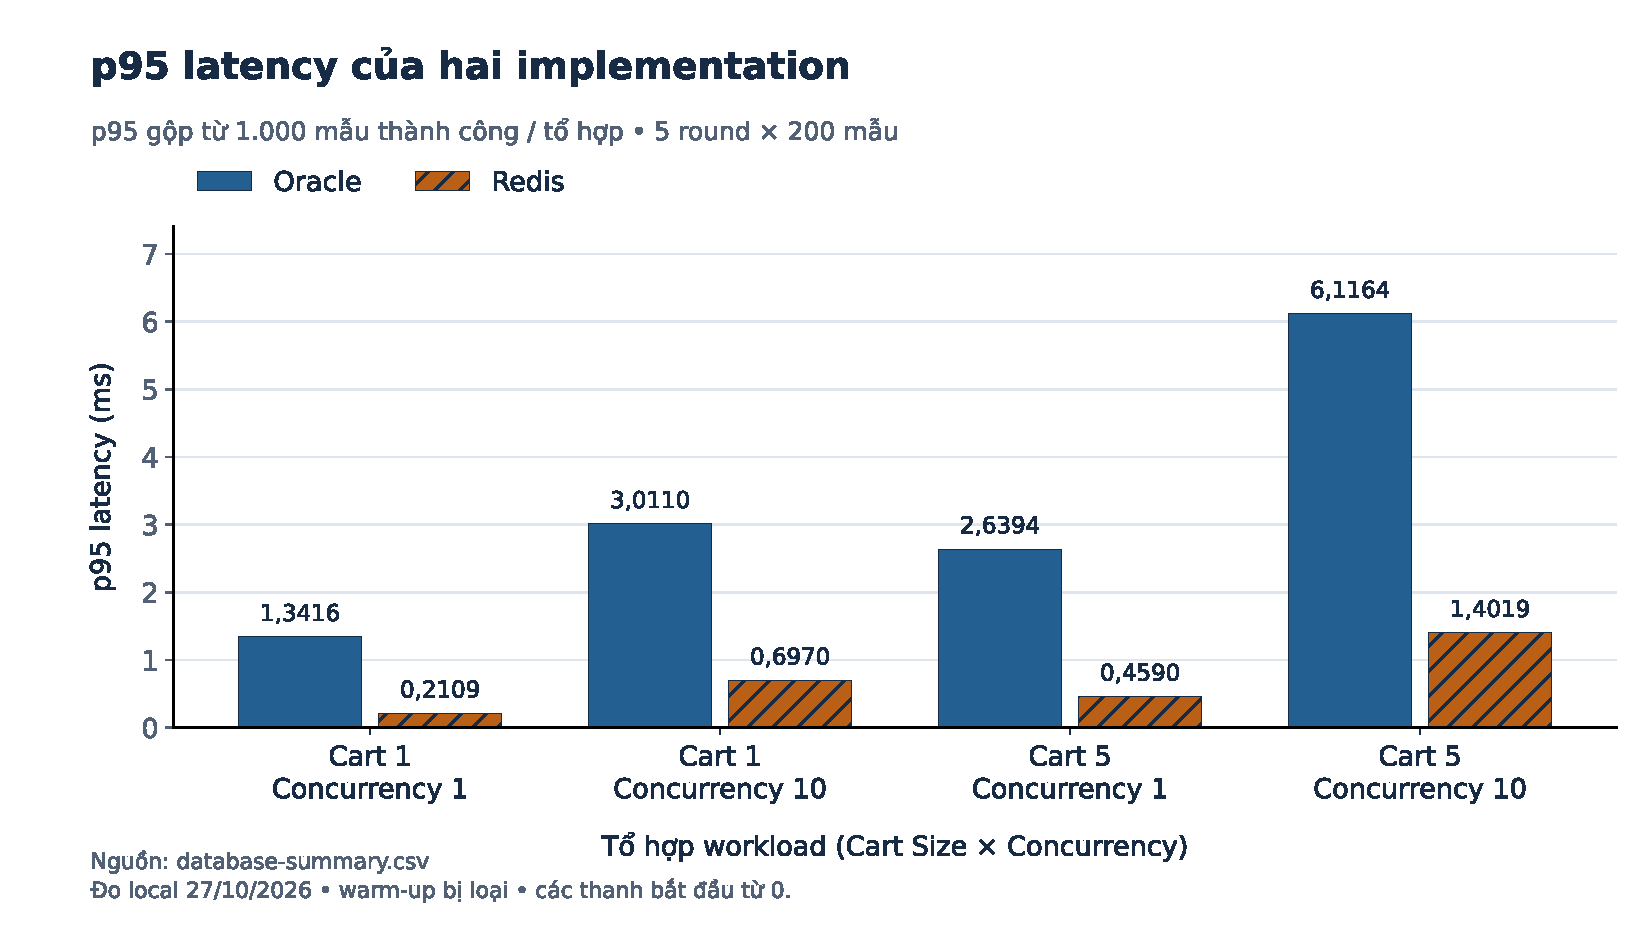
\includegraphics[width=\linewidth]{transaction/images/4.3-01-database-p95.pdf}
\caption[So sánh p95 latency Oracle–Redis theo Cart Size và Concurrency]{So sánh p95 latency Oracle–Redis theo Cart Size và Concurrency; dữ liệu từ bảng Database-level Benchmark, đơn vị ms.}\label{fig:tx-1}
\end{figure}
\begin{figure}[H]
\centering
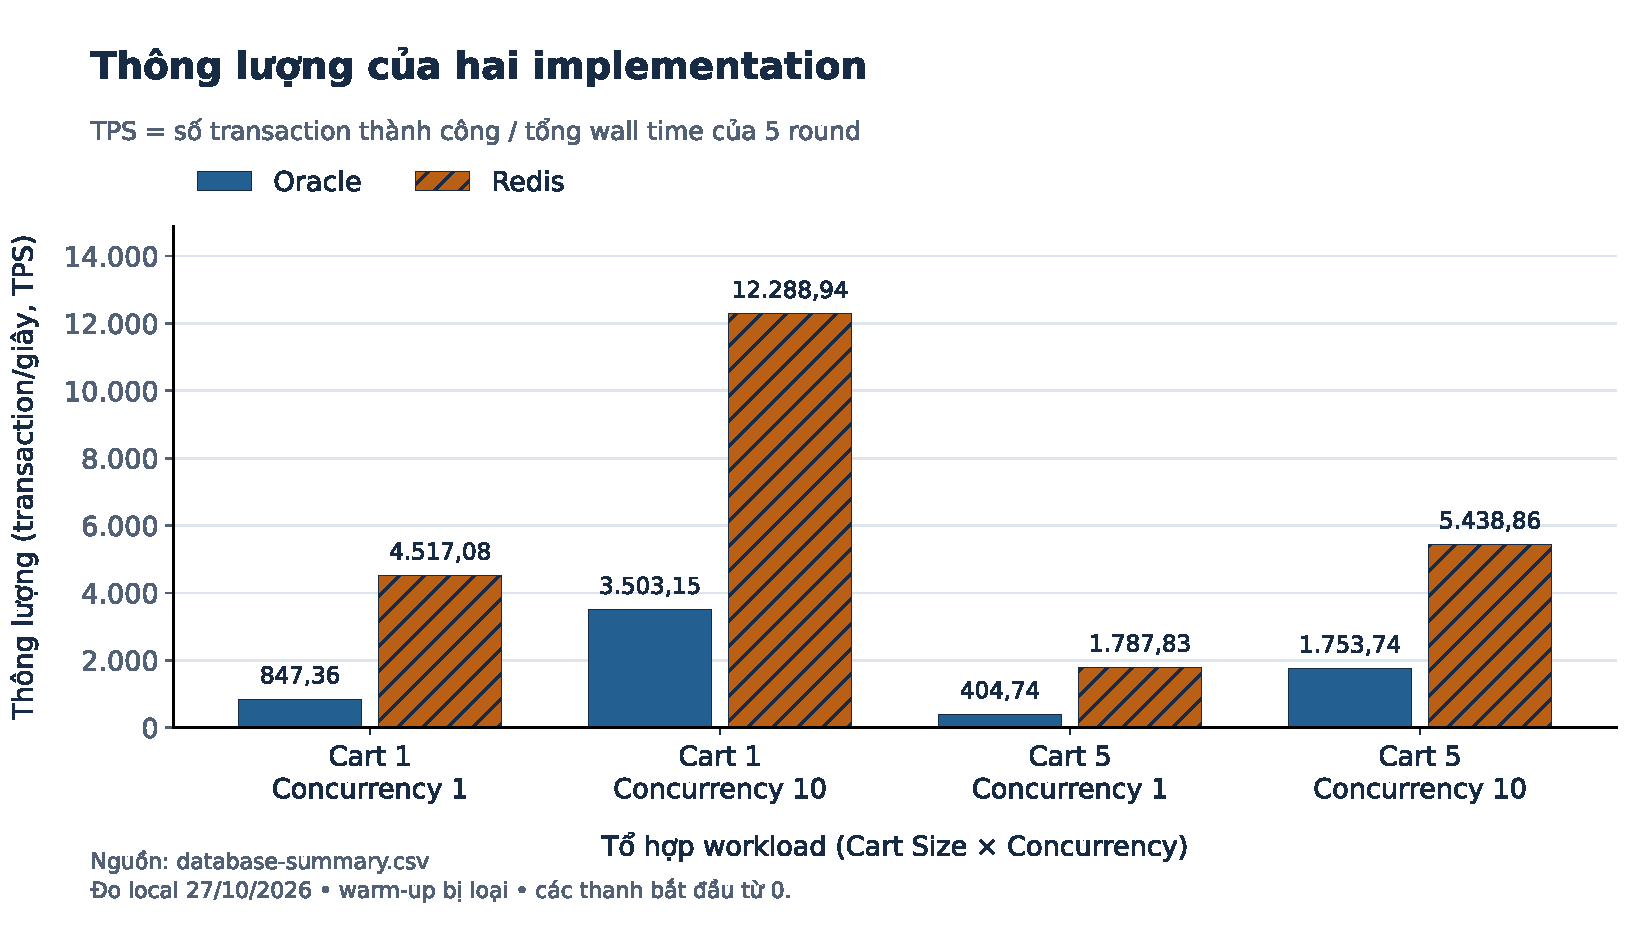
\includegraphics[width=\linewidth]{transaction/images/4.3-02-database-tps.pdf}
\caption[So sánh TPS Oracle–Redis theo bốn tổ hợp tải]{So sánh TPS Oracle–Redis theo bốn tổ hợp tải; dữ liệu từ bảng Database-level Benchmark.}\label{fig:tx-2}
\end{figure}
\textbf{Nhận xét kết quả.} Khi tăng Cart Size từ 1 lên 5, \textbf{p95 tăng và TPS giảm} ở cả hai implementation do một transaction phải xử lý nhiều dòng sản phẩm hơn. Khi tăng Concurrency từ 1 lên 10, \textbf{TPS tăng nhưng p95 cũng tăng}, phản ánh sự đánh đổi giữa thông lượng và thời gian xử lý từng giao dịch.

Redis có \textbf{p95 thấp hơn và TPS cao hơn trong cả bốn tổ hợp}. Ở Cart Size 5, Concurrency 10, Oracle đạt \textbf{6,1164 ms và 1.753,74 TPS}, trong khi Redis đạt \textbf{1,4019 ms và 5.438,86 TPS}. Kết quả này ghi nhận ưu thế của implementation Redis trong workload đã đo, nhưng chưa đủ để khẳng định Redis nhanh hơn Oracle đối với mọi transaction.

\begin{table}[H]
\centering
\caption{Trung bình và độ lệch chuẩn của p95 qua năm round. Nguồn: \texttt{results/\allowbreak{}summary-\allowbreak{}20261027/\allowbreak{}database-\allowbreak{}summary.\allowbreak{}csv}.}\label{tab:tx-13}
\footnotesize
\setlength{\tabcolsep}{3pt}
\renewcommand{\arraystretch}{1.2}
\begin{tabularx}{\linewidth}{@{}>{\hsize=0.65\hsize\linewidth=\hsize}L>{\hsize=0.85\hsize\linewidth=\hsize}L>{\hsize=1.25\hsize\linewidth=\hsize}L>{\hsize=1.25\hsize\linewidth=\hsize}L@{}}
\toprule
\textbf{Cart Size} & \textbf{Concurrency} & \textbf{Oracle p95 TB \(\pm\) SD (ms)} & \textbf{Redis p95 TB \(\pm\) SD (ms)} \\
\midrule
1 & 1 & 1,2784 \(\pm\) 0,2425 & 0,1869 \(\pm\) 0,0451 \\
1 & 10 & 3,0004 \(\pm\) 0,1745 & 0,7042 \(\pm\) 0,0370 \\
5 & 1 & 2,6187 \(\pm\) 0,0733 & 0,4494 \(\pm\) 0,0388 \\
5 & 10 & 5,7613 \(\pm\) 0,5800 & 1,3381 \(\pm\) 0,2104 \\
\bottomrule
\end{tabularx}
\end{table}
Chênh lệch giữa các round không đảo ngược xu hướng hiệu năng trên. Toàn bộ \textbf{8.000/8.000 transaction thành công}, không phát hiện invariant violation trong phạm vi hậu kiểm. Tuy nhiên, fixture chủ yếu độc lập giữa các worker, nên benchmark \textbf{chưa đo mức tranh chấp cao trên cùng sản phẩm}; khác biệt về schema, kết nối và durability cũng cần được xét khi diễn giải kết quả.

\txsubsection{Kết quả Application-level Benchmark}\label{sec:tx-3-3}
Phép đo HTTP sử dụng \textbf{k6 \(\rightarrow\) Vite proxy \(\rightarrow\) Spring Boot \(\rightarrow\) Oracle}, nhằm quan sát hiệu năng nghiệp vụ thực tế, \textbf{không so sánh Oracle với Redis ở tầng ứng dụng}. Một flow gồm đọc Cart, thêm 1 hoặc 5 sản phẩm, xem Checkout Preview, tạo Order, truy vấn danh sách/chi tiết Order và hủy Order. Do đó, \textbf{4.000 flow} tương ứng \textbf{36.000 HTTP request nghiệp vụ} (7 request/flow với Cart Size 1; 11 request/flow với Cart Size 5), không tính warm-up và login.

Bảng kết quả phân biệt \textbf{Checkout API} — riêng request tạo Order — với \textbf{Full Flow} — toàn bộ chuỗi thao tác nói trên.

\begin{table}[H]
\centering
\caption{Kết quả Application-level Benchmark. Latency lấy từ các mẫu thành công; Flow/s tính theo số flow thành công trên tổng thời gian thực của năm round. Nguồn: \texttt{results/\allowbreak{}summary-\allowbreak{}20261027/\allowbreak{}http-\allowbreak{}summary.\allowbreak{}csv}.}\label{tab:tx-14}
\scriptsize
\setlength{\tabcolsep}{3pt}
\renewcommand{\arraystretch}{1.2}
\begin{tabularx}{\linewidth}{@{}>{\hsize=0.65\hsize\linewidth=\hsize}L>{\hsize=0.9\hsize\linewidth=\hsize}L>{\hsize=1.1\hsize\linewidth=\hsize}L>{\hsize=1.1\hsize\linewidth=\hsize}L>{\hsize=1.15\hsize\linewidth=\hsize}L>{\hsize=1.15\hsize\linewidth=\hsize}L>{\hsize=0.95\hsize\linewidth=\hsize}L@{}}
\toprule
\textbf{Cart Size} & \textbf{Concurrency} & \textbf{Checkout p50 (ms)} & \textbf{Checkout p95 (ms)} & \textbf{Full Flow p50 (ms)} & \textbf{Full Flow p95 (ms)} & \textbf{Flow/s} \\
\midrule
1 & 1 & 2,9084 & 4,0406 & 14 & 18 & 68,34 \\
1 & 10 & 6,5273 & 8,9241 & 33 & 42 & 296,08 \\
5 & 1 & 4,9161 & 10,2897 & 30 & 62 & 27,73 \\
5 & 10 & 11,1444 & 14,7888 & 61 & 74 & 157,57 \\
\bottomrule
\end{tabularx}
\end{table}
\begin{figure}[H]
\centering
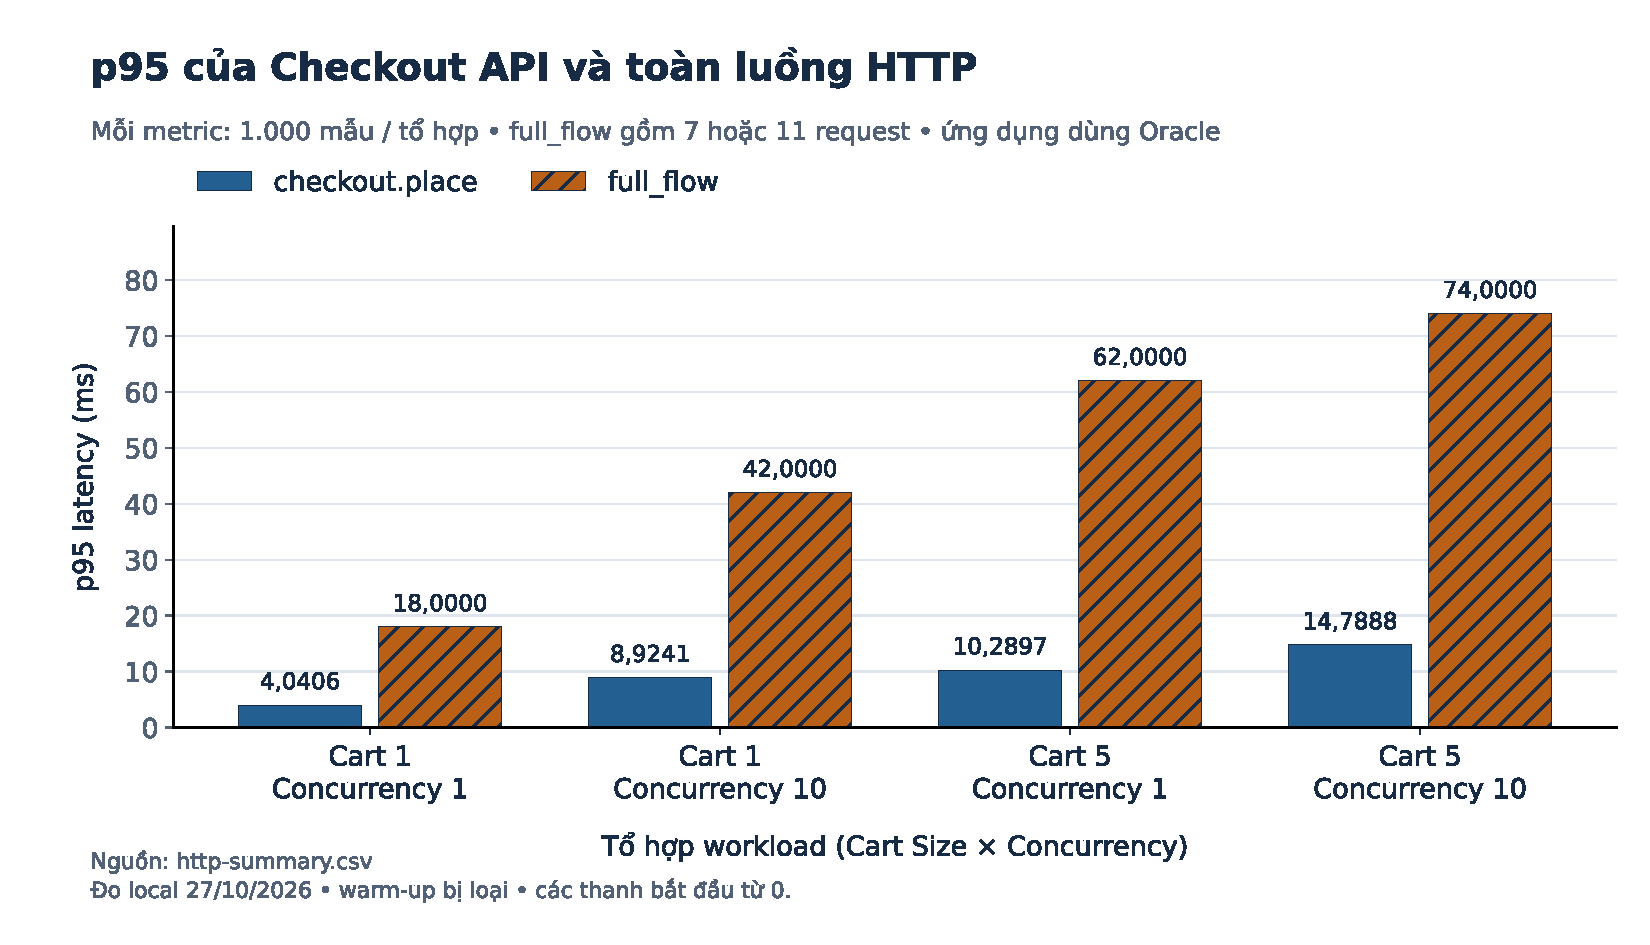
\includegraphics[width=\linewidth]{transaction/images/4.3-03-http-p95.pdf}
\caption[So sánh p95 Checkout API và Full Flow theo Cart Size/\allowbreak{}Concurrency]{So sánh p95 Checkout API và Full Flow theo Cart Size/\allowbreak{}Concurrency; dữ liệu từ bảng HTTP benchmark, đơn vị ms.}\label{fig:tx-3}
\end{figure}
\textbf{Nhận xét kết quả.} Khi Cart Size tăng từ 1 lên 5 ở Concurrency 1, Checkout p95 tăng từ \textbf{4,0406 lên 10,2897 ms}, Full Flow p95 tăng từ \textbf{18 lên 62 ms}. Nguyên nhân là Checkout phải xử lý nhiều sản phẩm và flow có thêm các request thêm Cart Item. Khi Concurrency tăng từ 1 lên 10, throughput tăng ở cả hai Cart Size (tương ứng \textbf{68,34 \(\rightarrow\) 296,08} và \textbf{27,73 \(\rightarrow\) 157,57 flow/s}), nhưng latency cũng tăng.

\textbf{Full Flow p95 cao hơn Checkout p95} vì chứa nhiều bước nghiệp vụ; không thể lấy chênh lệch hai phân vị làm chi phí chính xác của những API còn lại. Cả \textbf{4.000/4.000 flow hoàn tất}, không phát hiện invariant violation theo hậu kiểm. Kết quả cho thấy backend Oracle vận hành được dưới các mức tải đã thử, nhưng môi trường local và việc chưa tạo tranh chấp mạnh không đủ để suy ra hiệu năng production. \textbf{TPS database và Flow/s HTTP không thể so sánh trực tiếp} do khác đơn vị công việc.

\txsubsection{Đối chiếu tổng hợp và lựa chọn DBMS phù hợp}\label{sec:tx-3-4}
Từ các thí nghiệm chức năng và benchmark, hai DBMS có điểm mạnh khác nhau:

\begin{table}[H]
\centering
\caption{Tổng hợp kết quả nghiên cứu Transaction trên Oracle và Redis.}\label{tab:tx-15}
\footnotesize
\setlength{\tabcolsep}{3pt}
\renewcommand{\arraystretch}{1.2}
\begin{tabularx}{\linewidth}{@{}>{\hsize=0.65\hsize\linewidth=\hsize}L>{\hsize=1.175\hsize\linewidth=\hsize}L>{\hsize=1.175\hsize\linewidth=\hsize}L@{}}
\toprule
\textbf{Tiêu chí} & \textbf{Oracle} & \textbf{Redis} \\
\midrule
\textbf{Atomicity} & Hỗ trợ COMMIT, ROLLBACK và SAVEPOINT; cho phép hoàn tác các thay đổi chưa commit trên nhiều bảng (A1, A3, D1). & MULTI/EXEC và Lua thực thi không bị command khác chen ngang, nhưng không tự hoàn tác những ghi thành công trước lỗi runtime (A4, A5). \\
\textbf{Consistency} & DBMS trực tiếp thực thi các constraint như PK, FK, UNIQUE và CHECK (C1, A2). & Các ràng buộc nghiệp vụ giữa những key phải được kiểm tra và bảo vệ trong đường ghi, chẳng hạn Lua guarded Checkout (C2). \\
\textbf{Isolation và Concurrency} & READ COMMITTED, row lock và SELECT FOR UPDATE hỗ trợ kiểm soát truy cập đồng thời; có cơ chế phát hiện deadlock (B1–B3). & Atomic command, WATCH và Lua hỗ trợ xử lý xung đột; cần lựa chọn cơ chế phù hợp với từng thao tác (B4, B5). \\
\textbf{Durability} & Sử dụng Redo Log và cơ chế phục hồi transaction. & Hỗ trợ RDB/AOF; môi trường khảo sát sử dụng AOF \texttt{everysec}. Chưa thực hiện crash-recovery benchmark để so sánh trực tiếp. \\
\textbf{Hiệu năng} & Có latency cao hơn và TPS thấp hơn trong workload database đã đo. & Có latency thấp hơn và TPS cao hơn trong cùng các tổ hợp khảo sát, nhưng hai implementation chưa tương đương hoàn toàn về ràng buộc và chi phí thực thi. \\
\bottomrule
\end{tabularx}
\end{table}
Chênh lệch latency/TPS đo được nghiêng về Redis, nhưng benchmark chưa tương đương hoàn toàn về schema, cơ chế ghi và contention. Trong bối cảnh ShopFlash, yêu cầu nghiệp vụ chính là cập nhật đồng thời \textbf{Order, Order Item, Cart và Inventory} mà không để lại một trạng thái dang dở. Ngược lại, quota Flash Sale phù hợp hơn với các thao tác nguyên tử hoặc Lua trên số lượng key hạn chế. Vì vậy \textbf{tính phù hợp với nghiệp vụ quan trọng hơn việc chọn DBMS có số TPS cao nhất}.

\textbf{Đánh giá và quyết định đối với Oracle.} Các cơ sở lựa chọn là \textbf{full rollback nhiều bảng} (A1, A3, D1), \textbf{constraint được DBMS cưỡng chế} (A2, C1) và \textbf{row lock/SELECT FOR UPDATE} để bảo vệ quyết định dựa trên tồn kho (B1–B3). \textbf{Quyết định:} chọn \textbf{Oracle làm source of truth} cho User, Product, Cart, Order, Order Items và Inventory. Normal Checkout thực hiện tạo Order, cập nhật Inventory/Cart trong \textbf{một Oracle transaction}; Order Cancellation đồng thời cập nhật trạng thái đơn và hoàn tồn. Kết quả mua Flash Sale đã hoàn tất cũng được ghi nhận chính thức ở Oracle.

\textbf{Đánh giá và quyết định đối với Redis.} \textbf{Atomic command} và \texttt{WATCH} (B4), cùng \textbf{Lua kiểm tra–ghi không bị xen ngang} (B5, C2), phù hợp với bộ đếm/quota cần xử lý nhanh. Giới hạn không rollback khi runtime error sau ghi (A5) đòi hỏi validation và kiểm soát đường ghi. \textbf{Quyết định:} dùng Redis cho \textbf{Flash Sale runtime}, quota, giới hạn theo user và \textbf{reservation tạm thời}; Product/Search và Analytics là dữ liệu dẫn xuất, không thay thế bản ghi giao dịch gốc tại Oracle.

\textbf{Kết luận:} ShopFlash chọn \textbf{Oracle làm DBMS giao dịch chính, Redis làm thành phần runtime bổ trợ}. Hai hệ không sử dụng distributed transaction/XA; khi Redis đã giữ suất nhưng Oracle rollback, thiết kế cần \textbf{bù trừ reservation}, còn dữ liệu dẫn xuất được đồng bộ sau Oracle COMMIT. Đây là \textbf{quyết định kiến trúc dựa trên kết quả nghiên cứu}, chưa phải bằng chứng rằng quy trình phối hợp Oracle–Redis đã được kiểm thử end-to-end trong bộ thí nghiệm.

\endgroup


\newpage
\section{Thiết kế và hiện thực ứng dụng}\label{sec:thiet-ke}
% Mục 4.1. Phần chung, nhóm tự phân công người viết.
\subsection{Kiến trúc chung}\label{sec:kien-truc}
\chuaviet{}

\nhapmuc{storage/thiet-ke}{\subsection}{Module storage: F1, F2}
\nhapmuc{indexing/thiet-ke}{\subsection}{Module indexing: F3, F4}
\nhapmuc{query/thiet-ke}{\subsection}{Module query: F5, F6}
\nhapmuc{transaction/thiet-ke}{\subsection}{Module transaction: F7, F8, F10 và đăng nhập}
\nhapmuc{concurrency/thiet-ke}{\subsection}{Module concurrency: F9}
\nhapmuc{backup-recovery/thiet-ke}{\subsection}{Module backup: F11}

\newpage
\section{Đánh giá và lựa chọn DBMS}\label{sec:danh-gia}
% Mục 5. Đánh giá và lựa chọn DBMS. Phần chung, nhóm tự phân công người viết.
\chuaviet{}


\newpage
\section{Kết luận và tự đánh giá}\label{sec:ket-luan}
% Mục 6. Kết luận và tự đánh giá. Phần chung, nhóm tự phân công người viết.
\chuaviet{}


% =============================================================================
% TÀI LIỆU THAM KHẢO (IEEE, chỉ in tài liệu được \cite)
% =============================================================================
\newpage
\phantomsection
\printbibliography[title={Tài liệu tham khảo}, heading=bibintoc]

% =============================================================================
% PHỤ LỤC A--D
% =============================================================================
\newpage
\phantomsection
\section*{Phụ lục}
\addcontentsline{toc}{section}{PHỤ LỤC}
% Tăng bộ đếm mục để liên kết trong PDF của phụ lục không trùng với các mục 7.x.
\stepcounter{section}
\setcounter{subsection}{0}
\renewcommand\thesubsection{\Alph{subsection}}

\subsection{Đóng góp của từng thành viên}\label{pl:dong-gop}
% Phụ lục A. Đóng góp của từng thành viên. Mỗi người tự điền dòng của mình.
\begin{table}[H]
\centering
\caption{Phân công và mức độ đóng góp}\label{tab:dong-gop}
\small
\renewcommand{\arraystretch}{1.3}
\begin{tabularx}{\linewidth}{|c|l|L|c|}
\hline
\textbf{MSSV} & \textbf{Họ và tên} & \textbf{Công việc} & \textbf{Đóng góp} \\ \hline
 & & & \\ \hline
 & & & \\ \hline
 & & & \\ \hline
 & & & \\ \hline
 & & & \\ \hline
\end{tabularx}
\end{table}


\subsection{Biên bản họp nhóm}\label{pl:bien-ban}
% Phụ lục B. Biên bản họp nhóm.
% Biên bản dạng PDF: đặt vào chung/bien-ban/ rồi dùng \includepdf[pages=-]{chung/bien-ban/hop-01.pdf}
\chuaviet{}


\subsection{Câu SQL và lệnh Redis}\label{pl:lenh}
\nhapmuc{storage/lenh}{\subsubsection}{Data storage and management}
\nhapmuc{indexing/lenh}{\subsubsection}{Indexing}
\nhapmuc{query/lenh}{\subsubsection}{Query processing}
\nhapmuc{transaction/lenh}{\subsubsection}{Transaction}
\nhapmuc{concurrency/lenh}{\subsubsection}{Concurrency control}
\nhapmuc{backup-recovery/lenh}{\subsubsection}{Data backup and recovery}

\subsection{Hướng dẫn chạy demo}\label{pl:chay-demo}
% Phụ lục D. Hướng dẫn chạy demo. Phần chung, nhóm tự phân công người viết.
\chuaviet{}


\end{document}
